\documentclass[10 pt]{article}
\usepackage[a4paper, total={7in, 9.5in}]{geometry}
\usepackage[spanish]{babel}
\usepackage{csquotes}
\usepackage{graphicx} 
\usepackage{caption}
\usepackage{hyperref}
\usepackage{graphicx}
\usepackage{float}
\usepackage{url}
\usepackage{color}
\usepackage{siunitx}
\usepackage{hhline}
\usepackage{multirow}
\usepackage[round]{natbib}
\bibliographystyle{plainnat}
\usepackage{todonotes}
\linespread{1.5}
\usepackage{imakeidx}
\makeindex[columns=3, title=Alphabetical Index, intoc]
\usepackage{amsmath}
\usepackage{multicol}
\usepackage{amsmath}


\begin{document}


\begin{titlepage}

    \begin{center}
    \vspace*{-0.5in}
    \begin{figure}[htb]
    \begin{center}
    
\includegraphics[scale=.3]{images/uba2.jpg}
    \end{center}
    \end{figure}
    
    \begin{large}
    Especialización en Explotación de Datos y Descubrimiento del Conocimiento\\
    \vspace*{0.15in}
    Facultad de Ciencias Exactas y Naturales \\
    \vspace*{0.15in}
    Universidad de Buenos Aires \\
    
    \vspace*{0.6in}
    \end{large}
    
    \begin{large}
    Trabajo integrador\\

    \vspace*{0.15in}
    Clasificación e imputación de datos faltantes utilizando máquinas de soporte vectorial en datos de llamados para reportar violencia sexual a la línea 137 \\
    
    
    \end{large}
    \vspace*{0.2in}
    \vspace*{0.3in}
    
    
    \vspace*{0.3in}
    \rule{80mm}{0.1mm}\\
    \vspace*{0.1in}
    \begin{large}
    María Victoria Colombo
    
    \vspace*{0.3in}
    
    \vspace*{0.1in}.01.2025
    \end{large}
    \end{center}
    
    \end{titlepage}

\newpage

\begin{abstract}
    En las estadísticas sobre violencia sexual, las dificultades para recolectar datos a menudo resultan en información faltante. En este trabajo analizo llamados a la línea nacional 137 para reportar situaciones de violencia sexual. Con particular foco en la situación convivencial entre la víctima y su agresor, utilizo NMDS para buscar agrupamientos visuales en los casos según esta variable. Luego, implemento SVM con el objetivo de imputar los datos faltantes en la variable. Experimento con dos tipos de preprocesamientos para entrenar los clasificadores: uno con NMDS, y uno manual. Las visualizaciones con NMDS no resultan informativas. El preprocesamiento manual obtiene los mejores resultados en SVM. Sin embargo, el desbalance de las clases en la variable objetivo afecta largamente la performance del clasificador.  
\end{abstract}
\newpage
\tableofcontents
\newpage

\section{Introducción}\label{intro}

\subsection{Antecedentes}


La violencia sexual comprende una multiplicidad de conductas o intentos de conductas dirigidos contra la sexualidad de otra persona de manera coercitiva. Los datos sobre violencia sexual suelen ser escasos o presentar gran cantidad de faltantes \citetext{\citealp[p.~150]{ferris2002world}}. Uno de los motivos es que las víctimas o su entorno a menudo se rehúsan a denunciar o reportar estas situaciones, o proveen información incompleta. Esto puede deberse a la vergüenza y el estigma social frecuentemente asociado no solo con la violencia sexual sino con la sexualidad en general; pero también a la falta de acceso a la justicia, al temor a las represalias por parte de los agresores, o al temor a que la denuncia no sea creída \citetext{\citealp{murphy2022unfounded}}. Otros posibles motivos para la escasez y/o mala calidad de los datos pueden ser la falta de vías adecuadas para recabar esta información, o la negligencia o desconocimiento de procedimientos adecuados por parte de oficiales encargados de recibir denuncias. 

A pesar de estas dificultades, diversos estudios a nivel mundial logran identificar patrones en la violencia sexual. Dos de los más frecuentes son: la mayoría de las víctimas son mujeres, mientras que los perpetradores suelen ser hombres \citetext{\citealp[p.~149]{ferris2002world}; \citealp[p.~15]{contreras2016violencia}}; y en la mayoría de los casos, los agresores son personas conocidas por las víctimas, como parejas, exparejas u otros conocidos \citetext{\citealp[p.~9]{garcia2005multi},\citealp[p.~22]{unicef2018analisis}, \citealp[p.~151]{ferris2002world}}.
 
La clasificación de las identidades de género de víctimas y perpetradores es más compleja de lo que parece. Por un lado, muchos estudios clasifican a las personas únicamente como hombres o mujeres, omitiendo las identidades de género disidentes.\footnote{Entre los estudios e informes consultados para este trabajo, solamente el \textit{Relevamiento de fuentes secundarias de datos sobre violencia sexual} de la \citet{ufem_relevamiento} menciona identidades de género cuando especifica que la violencia sexual “afecta particularmente a las mujeres cis y personas LGBTI+” (p.7).}. Por otro lado, es probable que los casos de violencia sexual contra hombres cis género estén subrepresentados debido a prejuicios y estigmas sociales que dificultan el acceso a la justicia para estas víctimas \citep*[p.~149]{ferris2002world}. En mi análisis las categorías de género de los sujetos se limitan a las registradas en el conjunto de datos con que trabajo: hombre, mujer, y transgénero, sin especificar si es un hombre o una mujer transgénero. Reconozco esto como una limitación no solo de mi trabajo sino también de los datos disponibles. 

La  recopilación, sistematización, y análisis de datos sobre violencia sexual por parte de los Estados es crucial para planificar y llevar adelante políticas efectivas de prevención, asistencia, y erradicación de la violencia sexual. En Argentina, si bien no hay un sistema estatal único y centralizado de este tipo de información, existen entidades judiciales y programas estatales que, además de ofrecer auxilio, asistencia y/o acceso a la justicia, recaban datos sobre violencia sexual, y mantienen un registro público de ellos. Unos de esos programas es Las Víctimas contra las Violencias. 

Desde el año 2016, en el marco del programa Las Víctimas contra las Violencias, dependiente del Ministerio de Justicia de la Nación, la línea 137 funciona las 24 horas del día para solicitar asistencia en casos de violencia sexual o familiar.\footnote{Además, desde 2020 cuenta también con el canal de \textit{Whatsapp} (54911) 3133-1000.} El programa cuenta con equipos de intervención de abogadas, psicólogas, y trabajadoras sociales. Al recibir una llamada solicitando asistencia se coordina el envío de equipos móviles para proveer a la víctima, en base a las necesidades del caso, de contención emocional, acompañamiento a un hospital y/o a radicar una denuncia, y/o acompañamiento a un lugar seguro donde pueda alojarse \citep*{linea_137}.

Los registros de las llamadas a la línea 137 se encuentran digitalizados desde 2017 y están disponibles en el \href{http://datos.jus.gob.ar/}{Portal de Datos Abiertos de la Justicia Argentina}. Allí se encuentran publicados cuatro tipos de \textit{datasets}: 

\begin{itemize}
    \item Llamados por situaciones de violencia familiar
    \item Llamados por situaciones de violencia sexual
    \item Intervenciones domiciliarias por situaciones de violencia familiar
    \item Intervenciones domiciliarias por situaciones de violencia sexual
\end{itemize}

En este trabajo, analizo los datos de llamados por situaciones de violencia sexual. Estos llamados presentan datos faltantes de dos maneras: celdas vacías en algunas variables numéricas, y respuestas no-sabe/no-contesta (en adelante \texttt{NS/NC}) en variables categóricas. Me resulta de particular interés la variable \texttt{victima\_convive\_agresor}, que codifica la situación convivencial entre la víctima y el agresor, y toma los valores \texttt{SI}, \texttt{NO}, y \texttt{NS/NC}. La información que provee esta variable puede ser crucial para determinar el tipo de asistencia y los pasos a seguir para asegurar el bienestar de la víctima. Teniendo en cuenta lo dicho al comienzo de la introducción sobre los desafíos para recopilar datos sobre violencia sexual, es probale que los datos faltantes en \texttt{victima\_convive\_agresor} estén relacionados con el motivo mismo por el que faltan. Sin embargo, determinar la razón por la que faltan es un desafío que no forma parte de este trabajo. 


\subsection{Objetivos}

Elegí -por su versatilidad para operar con variables de distinto tipo- la técnica de Escalamiento Multidimensional No Métrico\footnote{En adelante \textit{NMDS} por sus siglas en inglés \textit{Non-Metric Multidimensional Scaling}} para generar visualizaciones del conjunto de datos dos dimensiones y explorar agrupamientos entre las clases de la variable objetivo \texttt{victima\_convive\_agresor}. Luego, elegí entrenar Máquinas de Soporte Vectorial\footnote{en adelante \textit{SVM} por sus siglas en inglés \textit{Support Vector Machine}} por ser clasificadores con probado buen rendimiento tanto para datos lineales como no lineales, para imputar los datos faltantes en la variable objetivo experimentando con distintas estrategias de preprocesamiento. 


Mis objetivos generales para este trabajo son:

\begin{itemize}
    \item Ampliar y aportar al campo de las investigaciones en materia de violencia de género y violencia sexual en Argentina.
    \item Explorar los datos en busca de patrones de ordenamiento que distingan a los grupos de víctimas que conviven con su agresor de los que no.
    \item Entrenar un modelo predictivo de clasificación para imputar los datos faltantes en la variable \texttt{victima\_convive\_agresor}. 
    \item Contrastar y comparar distintos tipos de preprocesamientos de los datos para el entrenamiento del modelo predictivo según su impacto en el modelo final. 

\end{itemize}

Mis objetivos particulares:

\begin{itemize}
\item Visualizar las clases \texttt{SI}, \texttt{NO}, y \texttt{NS/NC} de la variable \texttt{victima\_convive\_agresor} utilizando la técnica de Escalamiento Multidimensional No Métrico.
\item Entrenar un modelo de Máquinas de Soporte Vectorial para completar los datos faltantes de la variable \texttt{victima\_convive\_agresor}.
\item Contrastar tipos de preprocesamientos de los datos para entrenar el modelo: 
\begin{itemize}
    \item Reducción mediante un reordenamiento con la técnica de NMDS.
    \item Reducción de los datos de manera manual, a través de la eliminación, agrupación y transformación de las variables respondiendo al conocimiento del dominio y los resultados de la exploración de los datos. 
    \item Eliminación de datos faltantes en variables numéricas.
    \item Imputación categórica de datos faltantes en variables numéricas. 
\end{itemize}
\item Evaluar y comparar el rendimiento de los diferentes modelos según el preprocesamiento de los datos utilizando diferentes métricas como precisión, cobertura, F1, y \textit{accuracy}.
    
\end{itemize}


Todo el código generado para este trabajo de especialización fue escrito en \textit{python} y puede encontrarse en el repositorio público: \url{https://github.com/VicColombo/linea_137_llamados_vs}


\section{Datos}\label{datos}

\subsection{Obtención y limpieza}\label{limpieza}
Descargué del \href{http://datos.jus.gob.ar/}{Portal de Datos Abiertos} mencionado arriba 5 conjuntos de datos en formato \textit{csv} de llamados a la línea 137 para reportar y solicitar asistencia por situaciones de violencia sexual. Los llamados pertenecen al período entre enero de 2017 y julio de 2021. 

Una vez descargados, unifiqué los 5 archivos en un solo conjunto de datos. Para eso fue necesario realizar una primera limpieza destinada a dejar consistentes los distintos archivos en términos de cantidad y nombre de columnas:

\begin{itemize}
    \item Eliminé la variable \texttt{caso\_id}, que solo existe a partir de 2020.
    \item Cambié el nombre de la variable \texttt{llamado\_provincia\_indec\_id} en los datos de 2017, 2018, y 2019 a su equivalente en 2020 y 2021: \texttt{llamado\_provincia\_id}.
\end{itemize}

El siguiente paso fue limpiar el conjunto de datos unificado de inconsistencias y errores de carga varios: 
\begin{itemize}
    \item Unifiqué para todas las variables pertinentes los valores \texttt{SI}, \texttt{NO}, y \texttt{NS/NC} dejándolos en mayúscula, ya que aparecían en distintos formatos: minúscula, mayúscula inicial, etc.
    \item Unifiqué en la variable \texttt{victima\_vinculo\_agresor} el valor \texttt{Ex pareja de la víctima} que aparecía también como \texttt{Ex pareja}, \texttt{Ex-pareja de la víctima} y \texttt{Expareja de la víctima}, otro tanto hice con \texttt{Pareja de la víctima} que presentaba variaciones similares.
    \item Unifiqué en \texttt{hecho\_lugar} dos variaciones de una misma categoría: \texttt{Otra institución}, y \texttt{Otra Institución}, optando por la primera forma.
    \item Sustituí todos los valores \texttt{Sin datos} por \texttt{NS/NC} por considerarlos equivalentes.
    \item Quité espacios de comienzo y final de \textit{strings} para solucionar problemas del tipo \texttt{Madre} =/= \texttt{  Madre} 
    \item Convertí en la variable \texttt{llamante\_vinculo} el valor \texttt{Vecino} a \texttt{Vecina/o}, ya que no necesariamente se refiere unívocamente a personas de género masculino.
    \item Unifiqué en \texttt{llamado\_provincia} “Ciudad Autónoma de Buenos Aires” y “CABA” optando por “CABA”. 
    \item Corregí en \textit{llamado\_provincia }las instancias de “Santa Fé” a “Santa Fe”.

\end{itemize}

\subsection{Análisis exploratorio}\label{exploración}

El conjunto de datos unificado consta de 19143 observaciones y 54 variables, en su mayoría categóricas, que aportan información sobre la víctima, el agresor, la persona que llama para reportar el hecho, el contexto del hecho y el tipo de violencia sufrida. En el cuadro \ref{tablavar} se puede ver un detalle de las variables y su tipo.

\begin{table}[H]
    \centering
    \small
    \caption{Resumen de las variables.}
    \label{tablavar}
    \begin{tabular}{|l|l|l|} 
    \hline
    \hline
    \multicolumn{1}{|c|}{\textbf{Descriptor}} & \multicolumn{1}{c|}{\textbf{Tipo variable}} & \multicolumn{1}{c|}{\textbf{Variable(s)}} 
    \\ 
    \hline
    \multirow{2}{*}{Víctima} & Cuantitativa & victima\_edad 
    \\ 
    \cline{2-3}
     & Cualitativa & \begin{tabular}[c]{@{}l@{}}victima\_genero, victima\_nacionalidad, victima\_discapacidad, \\ victima\_vinculo\_agresor, victima\_convive\_agresor, victima\_a\_resguardo\end{tabular}          
     \\ 
    \hline
    \multirow{2}{*}{Llamante} & Cuantitativa         & {llamante\_edad}             
    \\ 
    \cline{2-3}
     & Cualitativa& llamante\_genero, llamante\_vinculo                  
     \\ 
    \hline
    \multirow{2}{*}{Llamado}& Ordinal & llamado\_fecha\_hora                                            
    \\ 
    \cline{2-3} & Cualitativa & \begin{tabular}[c]{@{}l@{}} caso\_id, llamado\_provincia llamado\_provincia\_id, \\ caso\_judicializado, hecho\_lugar\end{tabular}                                
    \\ 
    \hline
    Violencia sexual                 & Cualitativa  &  \begin{tabular}[c]{@{}l@{}} vs\_violacion\_via\_vaginal, vs\_violacion\_via\_anal, vs\_violacion\_via\_oral, \\ vs\_tentativa\_violacion, vs\_tocamiento\_sexual, vs\_intento\_tocamiento, \\ vs\_intento\_violacion\_tercera\_persona, vs\_grooming, vs\_exhibicionismo, \\ vs\_amenazas\_verbales\_contenido\_sexual, vs\_explotacion\_sexual,\\ vs\_explotacion\_sexual\_comercial, vs\_explotacion\_sexual\_viajes\_turismo, \\ vs\_sospecha\_trata\_personas\_fines\_sexuales, \\ vs\_existencia\_facilitador\_corrupcion\_nnya, \\ vs\_obligacion\_sacarse\_fotos\_pornograficas, vs\_eyaculacion\_partes\_cuerpo, \\ vs\_acoso\_sexual, vs\_iniciacion\_sexual\_forzada\_inducida, \\ vs\_otra\_forma\_violencia\_sexual, vs\_no\_sabe\_no\_contesta \end{tabular} 
    \\ 
    \hline
    Otras violencias & Cualitativa & \begin{tabular}[c]{@{}l@{}} ofv\_sentimiento\_amenaza, ofv\_amenazas\_explicitas, ofv\_violencia\_fisica, \\ ofv\_intento\_ahorcar, ofv\_intento\_quemar,  ofv\_intento\_ahogar, \\ ofv\_amenaza\_muerte, ofv\_uso\_sustancias\_psicoactivas, \\ ofv\_intento\_privacion\_libertad, ofv\_privacion\_libertad, \\ ofv\_uso\_arma\_blanca, ofv\_uso\_arma\_fuego, ofv\_enganio\_seduccion,\\ ofv\_intento\_matar, ofv\_uso\_animal\_victimizar, ofv\_grooming, \\ ofv\_otra\_forma\_violencia, ofv\_no\_sabe\_no\_contesta\end{tabular} 
    \\ 
    \hline
    \end{tabular}
\end{table}

Las variables que describen la violencia sexual sufrida y otras formas de violencia reportadas pueden tomar los valores \texttt{SI} o \texttt{NO}, siendo este último el valor más común, como se aprecia más abajo en las figuras \ref{vssino} y \ref{ofvsino} que muestran la distribución de respuestas para violencia sexual y otras formas de violencia respectivamente. Es interesante notar el volumen de respuestas positivas de las categorías \texttt{vs\_no\_sabe\_no\_contesta} y \texttt{ofv\_no\_sabe\_no\_contesta}. Es decir, en gran cantidad de llamados se reporta una forma de violencia (sexual o no) sufrida, pero no se puede reportar qué forma. A lo largo de esta sección se observa esta prevalencia de respuestas de tipo \texttt{NS/NC} en casi todas las variables.

\begin{figure}[H]
\begin{center}
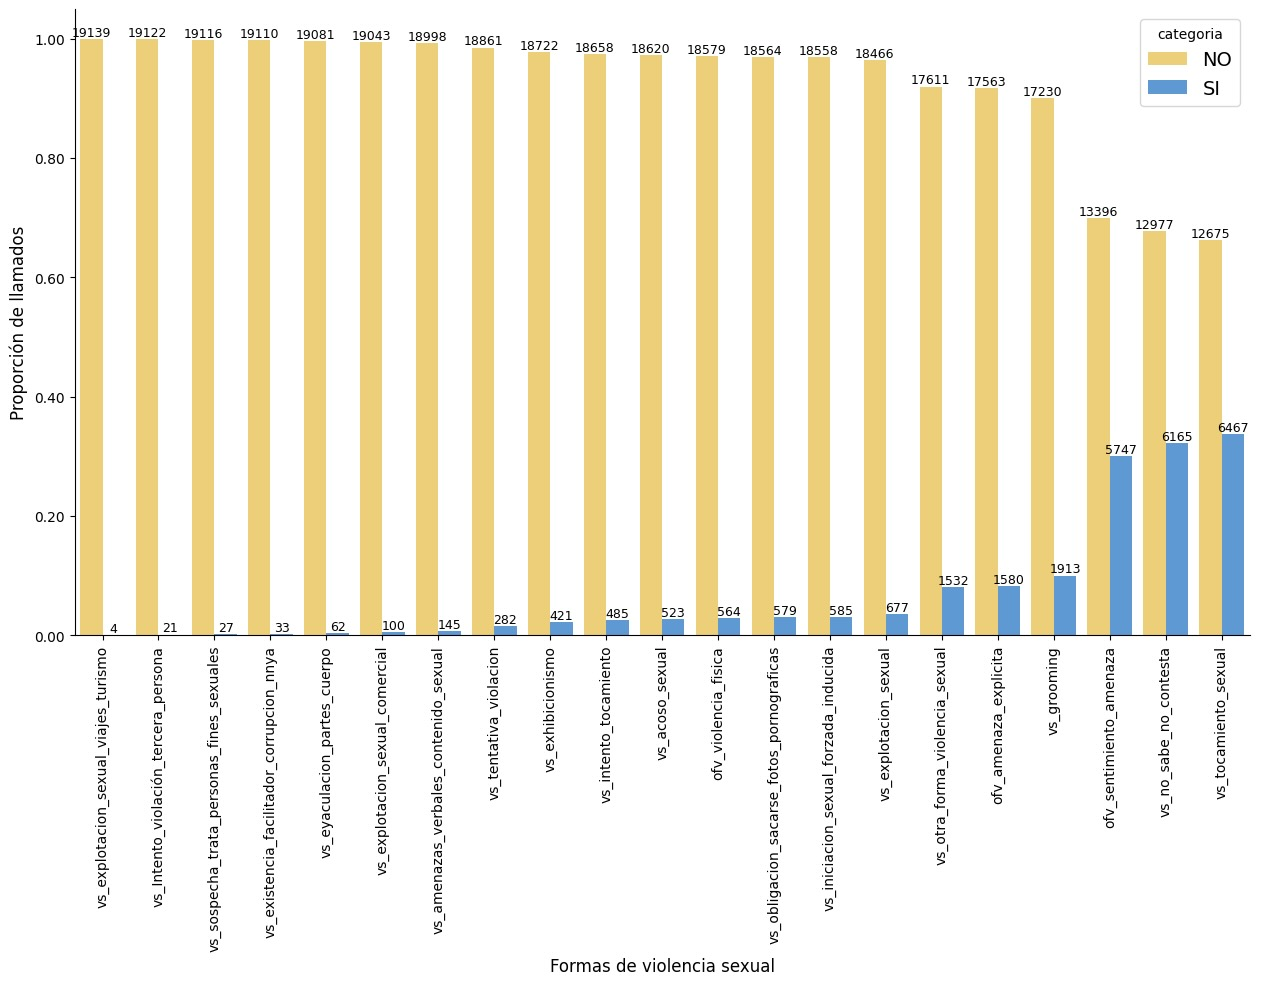
\includegraphics[scale=.4]{images/latex_vs_sino.jpeg}
\caption{Tipos de violencia sexual reportada.}
\label{vssino}
\end{center}
\end{figure} 

\begin{figure}[H]
\begin{center}
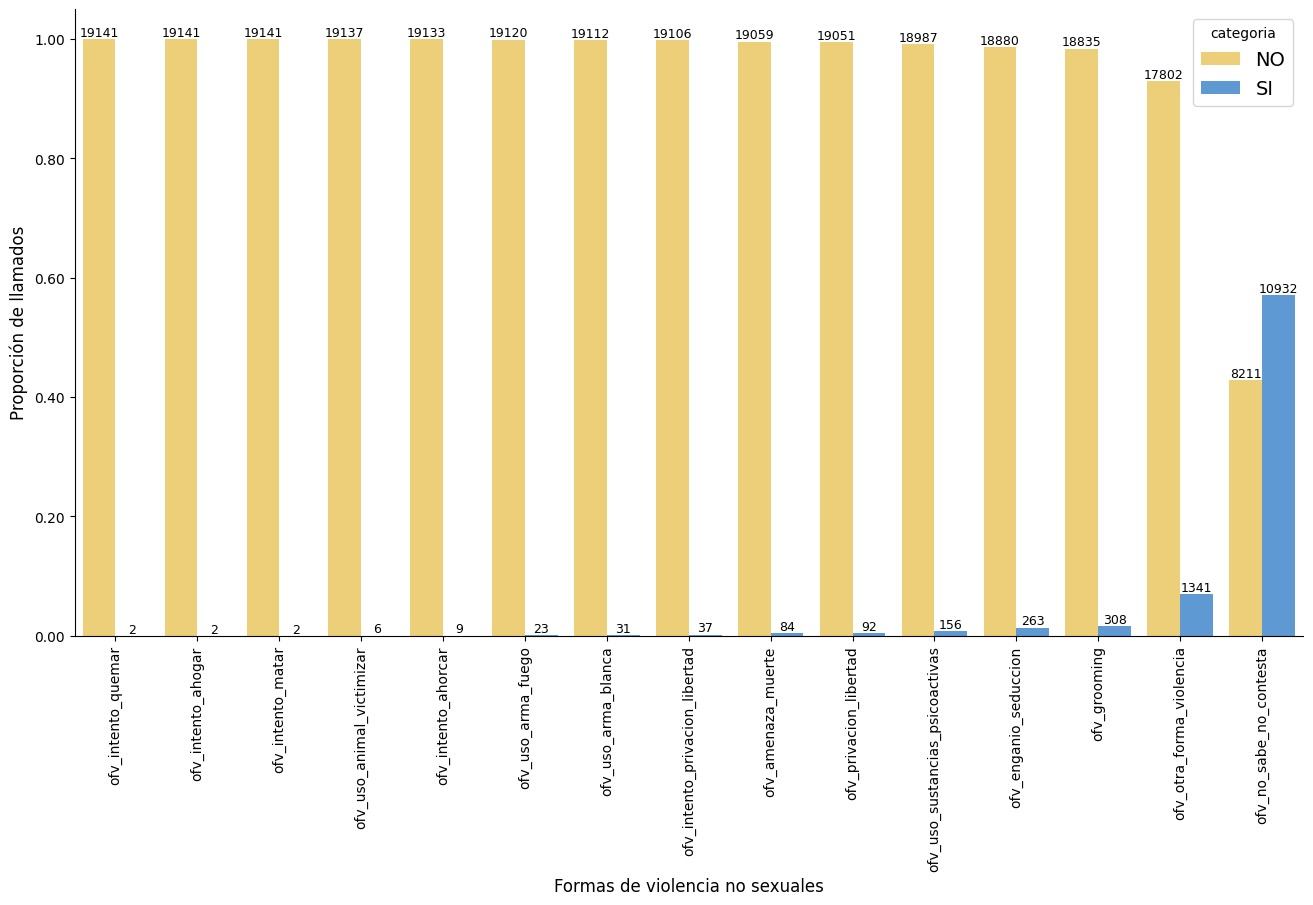
\includegraphics[scale=.4]{images/latex_ofv_sino.jpeg}
\caption{Tipos de violencia no sexual reportada.}
\label{ofvsino}
\end{center}
\end{figure} 



Las variables \texttt{victima\_edad} y \texttt{llamante\_edad} presentaban valores atípicos positivos, no solo identificables por superar la barrera de \(3*IQR\), sino también y principalmente por ser valores incongruentes con la edad de una persona. Por lo tanto, removí todos los valores por encima de 110 para ambas variables, y todos los valores por debajo de 1 para \texttt{llamante\_edad} (si existen víctimas que presentan edad 0, considero que se trata de menores que aún no alcanzan el año). Los valores removidos y su cantidad para cada variable pueden verse en el cuadro 2, \nameref{tabla_out}. Se puede comprobar allí que la mayoría eran 999 en ambas variables, muy probablemente un valor por defecto ingresado para no dejar el campo vacío. En total, removí 195 valores en \texttt{llamante\_edad}, y 101 valores en \texttt{victima\_edad}. 



\begin{table}[H]
    \centering
    \small
    \caption{Outliers en variables de edad.}
    \label{tabla_out}
    \begin{tabular}{lcc}
    \hline
    \multicolumn{1}{c}{\textbf{Variable}} & \textbf{Outlier} & \textbf{Cantidad de filas} \\ \hline
    \multirow{2}{*}{llamante\_edad}       & 999              & 192                        \\
                                          & 0                & 3                          \\ \hline
    \multirow{4}{*}{victima\_edad}        & 999              & 98                         \\
                                          & 224              & 1                          \\
                                          & 125              & 1                          \\
                                          & 111              & 1                          \\ \hline
    \end{tabular}
    \end{table}


Una vez removidos estos valores, tomé las medidas descriptivas de las variables de edad que se observan en el cuadro \ref{tabla_descr_ed}. Se puede ver que la mayoría de las víctimas no supera los 21 años, con una media de 17 y una moda de 14. Las personas que llaman para reportar los casos, en cambio, son en su mayoría adultos, con una media de 36 años, y una moda de 40. Esto refuerza lo mencionado en la introducción de hallazgos de otros estudios de que las personas más jóvenes y sobre todo los adolescentes e infantes son los grupos más en riesgo de ser víctimas de violencia sexual. 



    \begin{table}[H]
    \centering    
    \small
    \caption{Medidas descriptivas de las variables de edad.}
    \label{tabla_descr_ed}
        \begin{tabular}{lcc}    
        \hline
        \textbf{Descriptor} & \textbf{Edad de quien llama} & \textbf{Edad de la víctima} \\ \hline
        Media               & 36.25                        & 17.17                       \\
        Moda                & 40                           & 14                          \\
        Desvío Est.     & 11.41                        & 11.91                       \\
        Min.                & 3                            & 0                           \\
        25\%                & 29                           & 10                          \\
        50\%                & 35                           & 14                          \\
        75\%                & 42                           & 21                          \\
        Max                 & 99                           & 99                          \\ \hline
        \end{tabular}
        \end{table}


Para explorar patrones en la distribución temporal de los llamados realicé el gráfico de tendencia de la figura \ref{trend} con los datos agregados mensualmente y una media móvil de 4 meses. Se puede ver claramente en este gráfico una tendencia creciente en la cantidad de llamados desde mediados de 2017, que podría estar asociada a campañas de concientización sobre el programa y la línea y también sobre la violencia doméstica en general. Hay picos de llamados que se repiten alrededor de finales de cada año, entre los meses de octubre y enero en 2016, 2017, 2018 y 2020 aunque no parecen ser consistentes en tamaño como para considerarlos una tendencia clara. Por otro lado, hay una gran suba entre finales de 2018 y comienzos de 2019 que puede estar asociada a factores externos como los que mencioné antes. Se observa, luego de una baja y período de estabilización en 2019, una suba marcada en 2020. Un factor externo que podría estar relacionado con este patrón, es la implementación de políticas de ASPO (Aislamiento Social Preventivo y Obligatorio) durante la epidemia de COVID-19 de 2020 que obligó a la población a permanecer en sus hogares y entornos más cercanos. Si tenemos en cuenta la mayor prevalencia de la violencia sexual en ámbitos cercanos y por parte de agresores conocidos a la víctima, podría explicarse la suba de cantidad de llamados durante esta época. Sin embargo, cabe aclarar, que todas las posibles asociaciones que planteo como interpretación de esta figura deben ser contrastadas con un análisis en profundidad de las series temporales de los datos, que excede los objetivos de este trabajo.

\begin{figure}[H]
    \begin{center}
    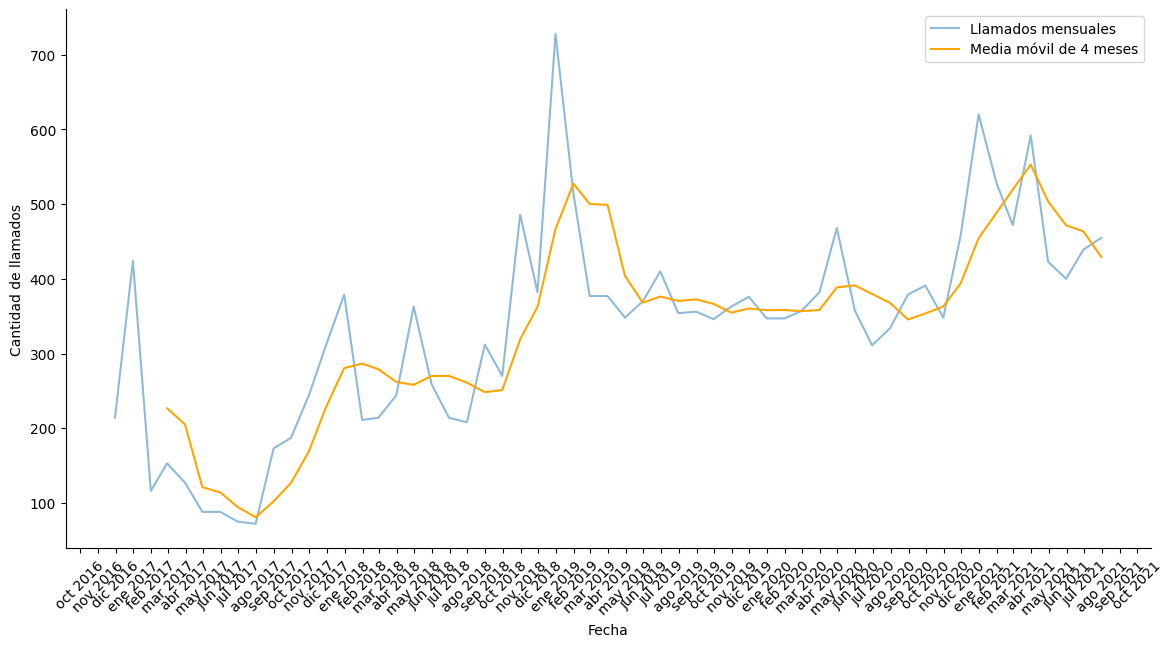
\includegraphics[scale=.4]{images/latex_trend_llamados.png}
    \caption{Cantidad de llamados en el tiempo con media móvil de 4 meses.}
    \label{trend}
    \end{center}
    \end{figure}

Además, construí las variables \texttt{estación del año}, \texttt{fin de semana}, y \texttt{momento del día} para explorar la posibilidad de otros patrones en los llamados. Observé que una mayor proporción de llamados ocurren durante la semana (80\%) y por la tarde (38\%). No observé disparidad significativa en la distribución de llamados de acuerdo a las estaciones del año.


Según la distribución de la variable \texttt{llamado\_provincia}, la mayoría de los llamados provienen de la Ciudad Autónoma (37\%) y la Provincia de Buenos Aires (36\%). Del 9\% no se cuentan con datos (respuestas \texttt{NS/NC}); y el restante 18\% se reparte entre las restantes provincias del país, siendo de ese grupo Córdoba y Santa Fé las que más llamados tienen, con un 3\% cada una.\footnote{Ver figura \ref{provincia} en el \nameref{anex}.}

Según la distribución de la variable \texttt{caso\_judicializado}, el 46.7\% de los llamados no está asociado a un caso ya judicializado, el 39.7\% sí, y en el restante 13.4\% no se cuenta con datos de este tipo.\footnote{Ver figura \ref{casojudicializado} en el \nameref{anex}.} 

En cuanto a la variable \texttt{hecho\_lugar}, como ilustra el gráfico de barras de la figura \Ref{hecholugar}, para aproximadamente el 30\% de los llamados no se cuenta con datos (respuestas \texttt{NS/NC}); luego, el 25\% los hechos suceden en la vivienda de la víctima y el 13\% en la vivienda del agresor. La cuarta categoría más reportada, con el 12\%, es \textit{redes sociales}. El restante 20\% se divide entre categorías de espacios públicos (plazas, descampados, etc.), transporte, y ámbito educativo, entre otros sitios. La elevada proporción de casos que suceden en la vivienda de la víctima, es un dato que acompaña lo ya dicho en la \nameref{intro} sobre la mayoría de los hechos de violencia sexual ocurriendo más bien en el entorno de la víctima antes que involucrar personas y lugares desconocidos. 

\begin{figure}[H]
    \begin{center}
    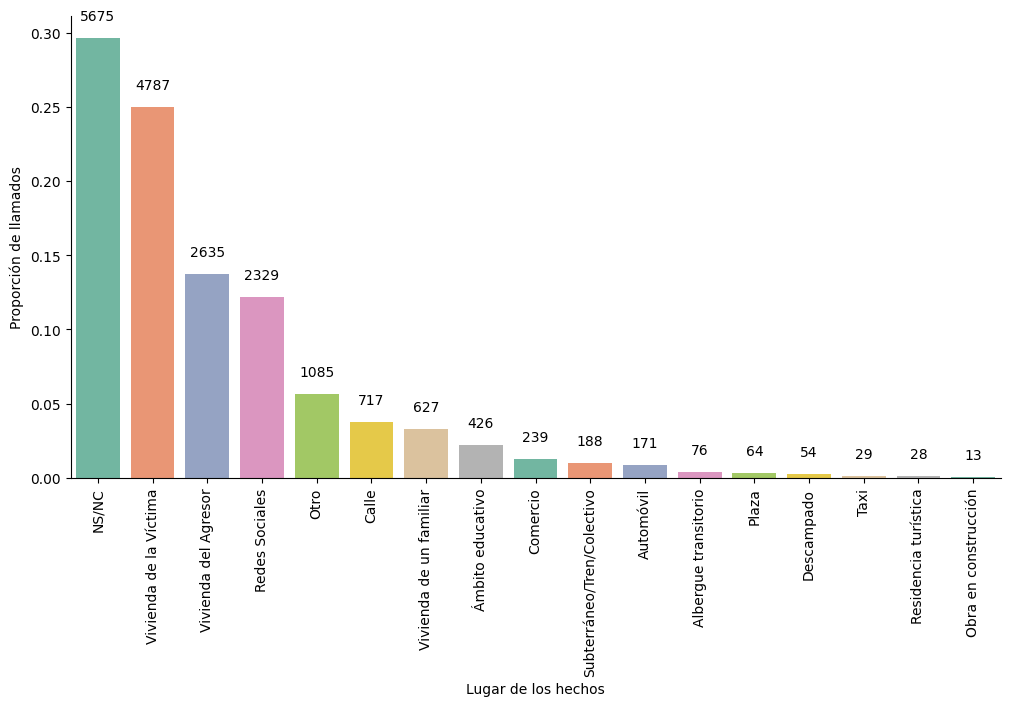
\includegraphics[scale=.4]{images/latex_lugar_hechos.png}
    \caption{Lugar de los hechos.}
    \label{hecholugar}
    \end{center}
    \end{figure}


Llama la atención la cuarta categoría más presente en \texttt{hecho\_lugar}, los casos sucedidos en redes sociales. Dada la media de edad de las víctimas que reporté más arriba, se podría hipotetizar sobre la relación entre estas variables: la población joven pasa más tiempo en redes sociales y entonces es más propensa a sufrir violencia sexual en ese lugar; o las redes sociales son lugares donde proliferan más los actos de violencia sexual por alguna(s) característica(s) intrínseca(s) de las redes mismas. 

%Para explorar este fenómeno, crucé en la figura \ref{redes}  esa categoría de \texttt{hecho\_lugar} con los tipos de violencia sufrida y las edades de las víctimas agrupadas cualitativamente en Niñez (0 a 11 años), Adolescencia (12 a 18 años), Juventud (19 a 30 años), Adultez (31 a 65 años), y Vejez (mayores de 65). Observé que la mayor cantidad de casos corresponden al tipo de violencia \textit{grooming} en primer lugar, y en segundo lugar a la categoría \textit{ofv\_no\_sabe\_no\_contesta}. Además, aunque con conteos mucho más bajos, aparecen también otras formas de violencia esperables en el contexto de redes sociales como: \textit{ofv\_sentimiento\_amenaza}, \textit{vs\_explotacion\_sexual}, o \textit{ofv\_amenaza\_explicita}. En todos estos casos alrededor del 90\% de las víctimas son niñes o adolescentes. Si bien por la distribución de la variable \texttt{victima\_edad} cabría esperar mayor cantidad de víctimas de estos grupos etarios, en el caso de los hechos sucedidos en redes sociales, este dato podría estar asociado con el mayor uso de redes sociales por parte de este sector de la población. 

%\begin{figure}[H]
%    \begin{center}
%    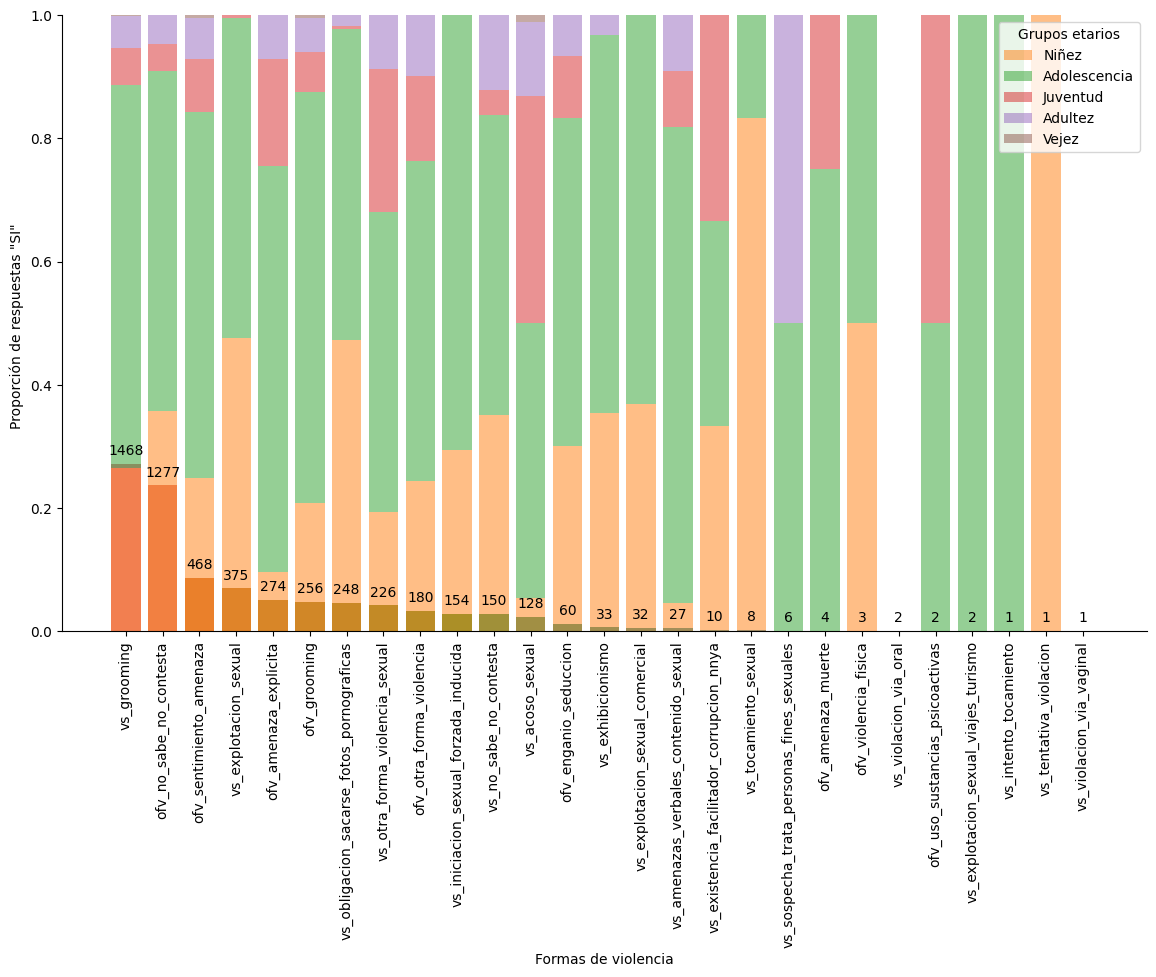
\includegraphics[scale=.5]{images/latex_redes_sociales_edad_formas_violencia.png}
%    \caption{Proporción de “SI” en hechos de violencia ocurridos en redes sociales, agrupado por edad.}
%    \label{redes}
%    \end{center}
%    \end{figure}


La nacionalidad de las víctimas, informada por \texttt{victima\_nacionalidad}, se distribuye de la siguiente manera: el 80\% de las víctimas son argentinas; del 15\% no se cuenta con datos; y el restante 5\% se divide entre las nacionalidades boliviana, paraguaya, peruana, brasileña, uruguaya, chilena, y la categoría “otra”.\footnote{Ver figura \ref{nacionalidad} en el \nameref{anex}}


Según la distribución de \texttt{victima\_discapidad}, para el 53.7\% de las víctimas no se cuenta con datos, el 43.2\% no posee discapacidad, y el 2.9\% sí\footnote{Ver figura \ref{discapacidad} en el \nameref{anex}}. 


En cuanto al género de las víctimas, en el gráfico de barras de la figura \Ref{genero}, se ve reforzado lo establecido en la Introducción sobre la distribución de género en las víctimas: el 77.6\% de las víctimas son mujeres, el 18.4\% hombres, del 3.7\% no se tienen datos, y el 0.14\% son personas transgénero. 

\begin{figure}[H]
    \begin{center}
    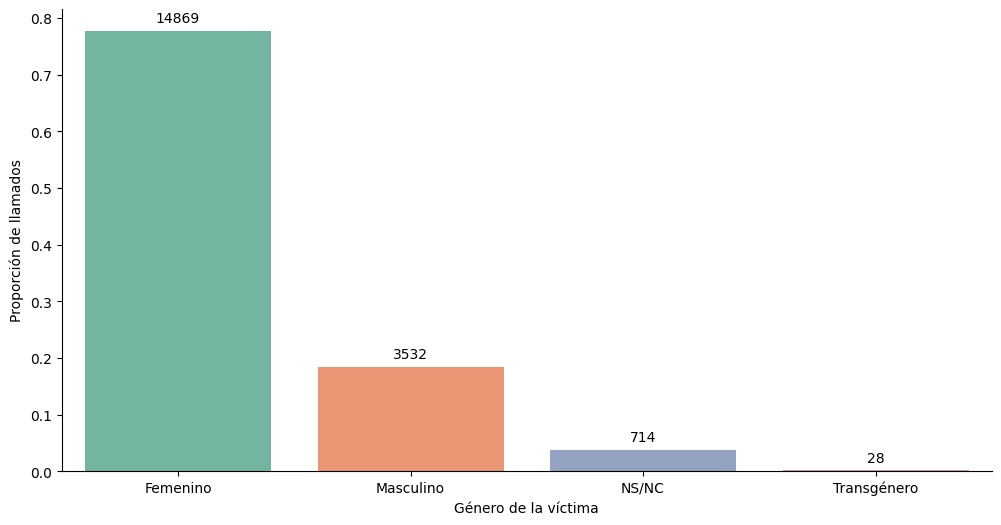
\includegraphics[scale=.4]{images/latex_genero_victima.png}
    \caption{Género de las víctimas.}
    \label{genero}
    \end{center}
    \end{figure}

Los vínculos entre víctimas y agresores nuevamente reflejan la persistencia de los hechos de violencia sexual perpetuados por personas del entorno de las víctimas. En el gráfico de barras de la figura \Ref{vinculoagresor} para la variable \texttt{victima\_vinculo\_agresor} se observa la distribución en las diferentes categorías vinculares. Pero además la tendencia se evidencia aún más al reagrupar las categorías de la variable en \texttt{Conocido familiar}, \texttt{Conocido no familiar} (categoría ya presente en la variable original) \texttt{Desconocido}, y \texttt{NS/NC}. Mientras que 15.4\% de los agresores son declarados como desconocidos; entre familiares (47.4\%) y no familiares (19.7\%), los agresores conocidos por la víctima suman un 67.1\%. El número podría incluso ser más elevado si consideramos que podría haber agresores conocidos también como parte del 17.2\% de los \texttt{NS/NC}.



\begin{figure}[H]
    \begin{center}
    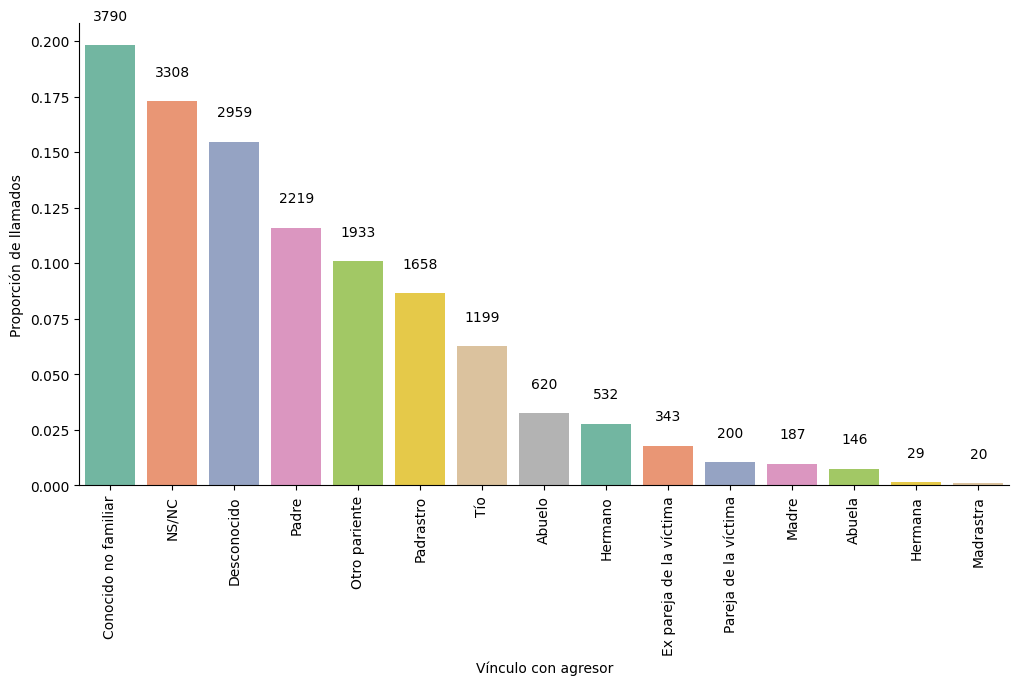
\includegraphics[scale=.4]{images/latex_vinculo_agr_victima.png}
    \caption{Vínculos víctima-agresor.}
    \label{vinculoagresor}
    \end{center}
    \end{figure}

    \begin{figure}[H]
        \begin{center}
        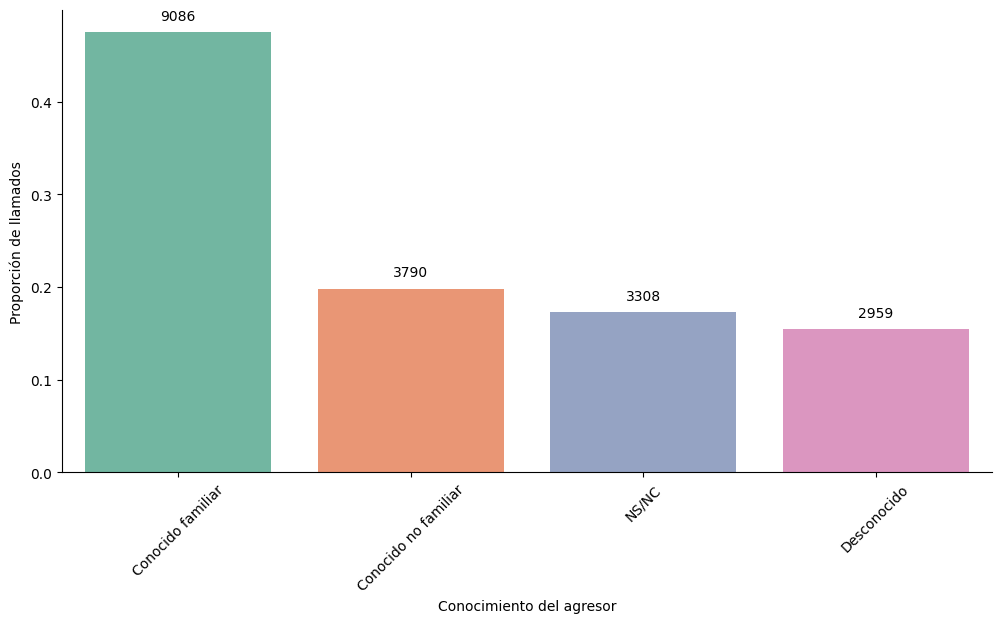
\includegraphics[scale=.4]{images/latex_agresor_conocido_no.png}
        \caption{Agresor conocido o no por la víctima.}
        \label{conocidodesconocido}
        \end{center}
        \end{figure}




 En la variable \texttt{vinculo\_llamante\_victima}, el 24.9\% de los llamados provienen de comisarías, el 17.2\% de un familiar de la víctima (otro familiar que no pertenezca a las categorías: \texttt{Madre}, \texttt{Padre}, \texttt{Abuela/o}, o \texttt{Hermana/o}), el 16\% de los llamantes son madres de las víctimas, y el 14.2\% lo constituyen las propias víctimas. El resto de las categorías son otros conocidos de las víctimas, padres, vecinos, abuelos, hermanos, otras instituciones, o \texttt{NS/NC} todas con menos del 10\%. Por último, los llamados provenientes de escuelas, defensorías y los mismos agresores suman menos del 1\%.\footnote{Ver figura \ref{vinculollamante} en el \nameref{anex}}



En cuanto a la variable de interés \texttt{victima\_convive\_agresor}, encontré en el análisis univariado que puede verse en el gráfico de barras de la figura \Ref{convivencia}, que quiénes sí conviven con su agresor son minoría, 14.3\%; mientras que el 64.4\% no convive con su agresor. El restante 21.19\% las respuestas son \texttt{NS/NC}, la categoría que más adelante intento predecir como \texttt{SI} o \texttt{NO}.  


\begin{figure}[H]
    \begin{center}
    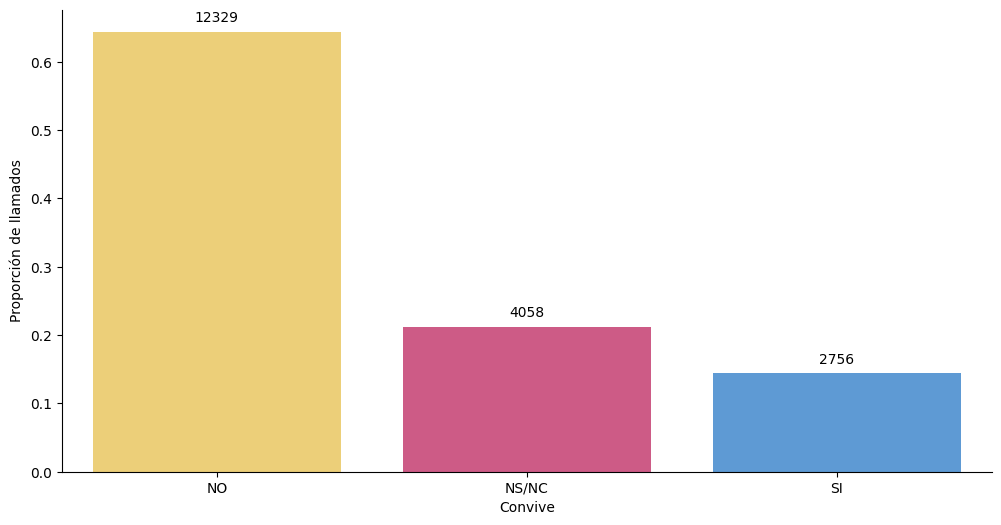
\includegraphics[scale=.4]{images/latex_convive.png}
    \caption{Convivencia víctima-agresor.}
    \label{convivencia}
    \end{center}
    \end{figure}


\subsubsection{Análisis multivariado de \texttt{victima\_convive\_agresor}}\label{faltantes}


Para un análisis multivariado seleccioné algunas variables que podían estar más relacionadas con 
\texttt{victima\_convive\_agresor}: \texttt{hecho\_lugar}, \texttt{momento\_dia}, \texttt{victima\_vinculo\_agresor}, \texttt{llamante\_vinculo}, y \texttt{victima\_edad}. 

Primero, realicé gráficos de barras para explorar la relación entre \texttt{victima\_convive\_agresor} y las variables categóricas.
Observé que la distribución original de \texttt{victima\_convive\_agresor} (mayoría de respuestas \texttt{NO} y minoría de \texttt{SI}, con \texttt{NS/NC} posicionado ordinalmente en el medio), se mantiene para casi todas las categorías de estas variables con las siguientes excepciones. En primer lugar, como se ve en la figura \ref{hecholugconvive}, cuando los hechos suceden en la vivienda de la víctima, hay más casos en los que la víctima sí convive con el agresor y la distribución pasa a ser \texttt{NO}, \texttt{SI}, \texttt{NS/NC}. Lo mismo sucede cuando los hechos ocurren en la vivienda del agresor, aunque en ese caso la proporción de \texttt{SI} supera por muy poco la proporción de \texttt{NS/NC}. 

En segundo lugar, en la figura \ref{agrvincconvive} se observa que para la mayor parte de los casos en los que el agresor es parte de la familia de la víctima (\texttt{Abuelo}, \texttt{Hermana}, \texttt{Hermano}, \texttt{Madrastra}, \texttt{Madre}, \texttt{Padrastro}, \texttt{Pareja de la víctima}), los casos en que la víctima convive son más que los casos en los que no hay respuesta sobre la situación convivencial. Sin embargo, solo en las categorías \texttt{Madre}, \texttt{Padrastro}, y \texttt{Pareja de la víctima} los casos en que las víctimas conviven con sus agresores superan a los casos en los que no lo hacen.

Por último, en la figura \ref{llamvincconvive}, se puede ver que para la categoría \texttt{vecina/o} de \texttt{llamante\_vinculo}, la tendencia de respuestas positivas y negativas también se invierte. Sobre esta variable se observa además que los valores de \texttt{NS/NC} para \texttt{victima\_convive\_agresor} son notablemente más altos cuando el llamado proviene de \texttt{Otra institución} que no sea una escuela, comisaría, u hospital. 


\begin{figure}[H]
\begin{center}
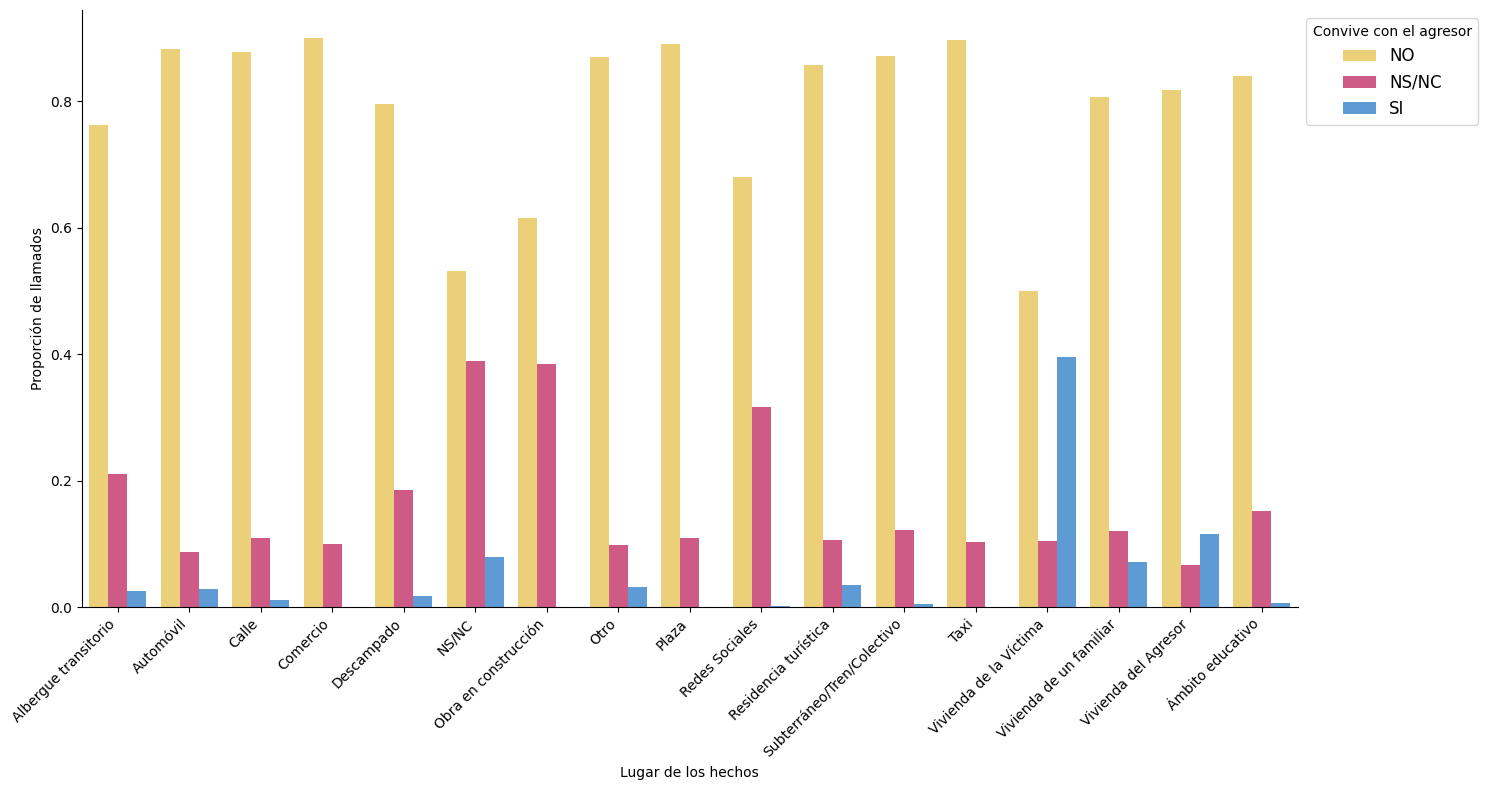
\includegraphics[scale=.4]{images/latex_hecho_lugar_convive.png}
\caption{Convivencia con el agresor según lugar de los hechos.}
\label{hecholugconvive}
\end{center}
\end{figure}
    
\begin{figure}[H]
\begin{center}
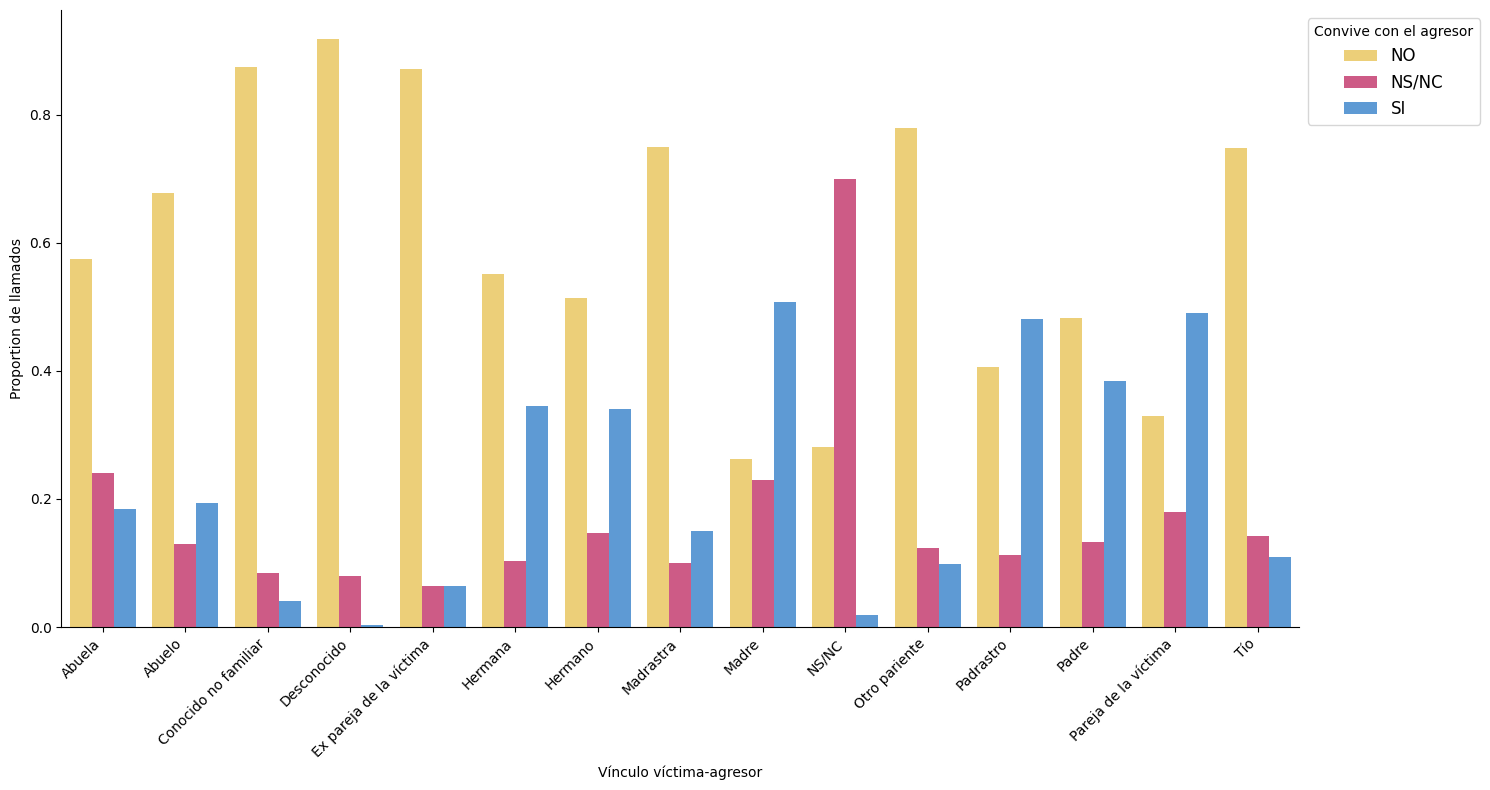
\includegraphics[scale=.4]{images/convive_vinc_agresor.png}
\caption{Convivencia con el agresor según vínculos víctima-agresor.}
\label{agrvincconvive}
\end{center}
\end{figure} 

\begin{figure}[H]
\begin{center}
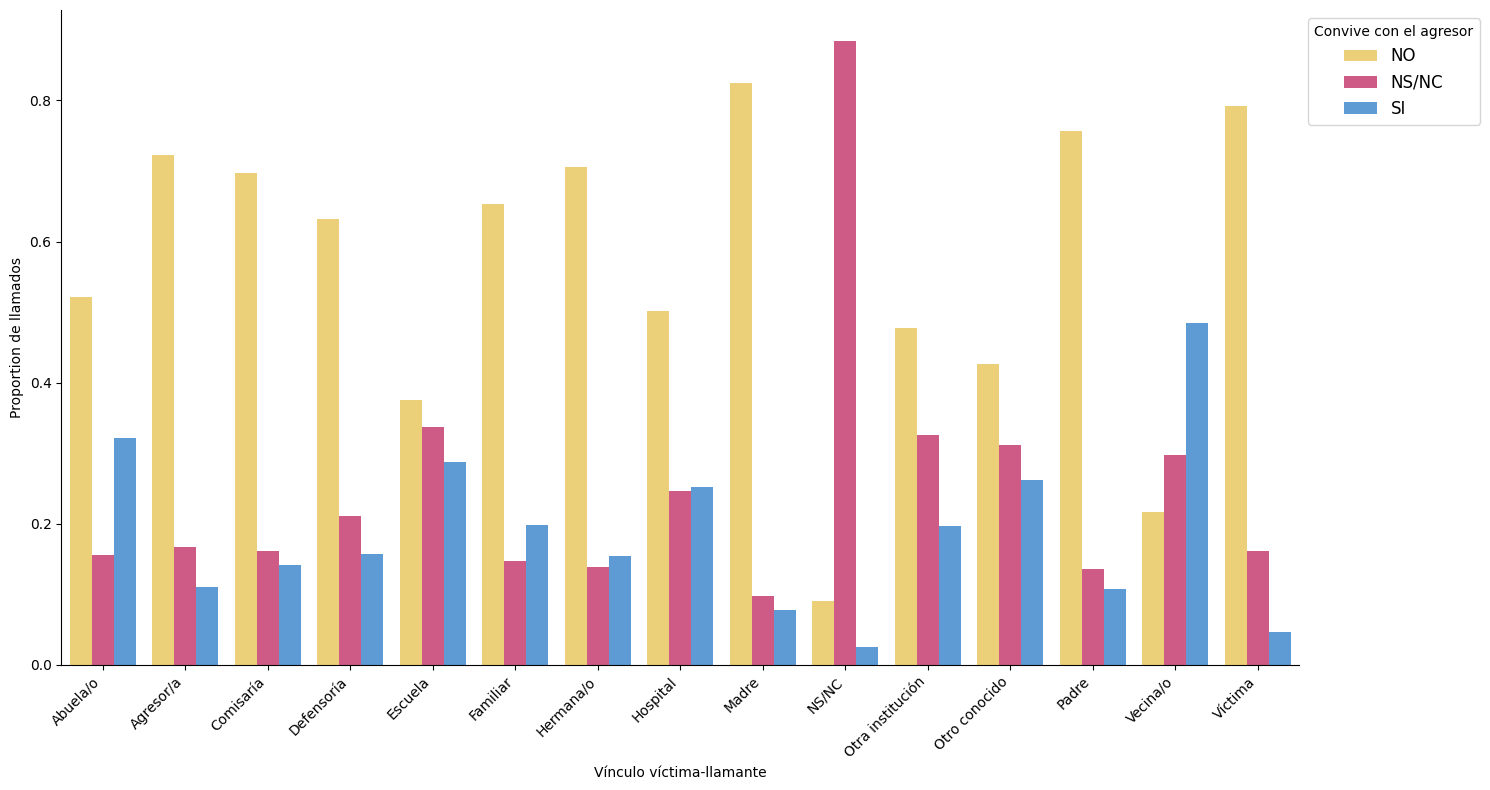
\includegraphics[scale=.4]{images/latex_llamante_vin_convive.png}
\caption{Convivencia con el agresor según vínculos víctima-llamante.}
\label{llamvincconvive}
\end{center}
\end{figure} 


Luego realicé \textit{boxplots} comparativos y un detalle del análisis de cuartiles de \texttt{victima\_edad} según cada categoría de \texttt{victima\_convive\_agresor}. Como se ve en la figura \ref{boxplotsconvivenciaedad} y el cuadro \ref{cuartilesconviveedad}, las víctimas que conviven con el agresor son ligeramente más jóvenes que las que no lo hacen; y las víctimas de las que no se cuenta con datos sobre la convivencia parecen estar más cerca en edad de las que conviven. Sin embargo, estas diferencias en edad no parecen significativas.

\begin{figure}[H]
    \begin{center}
    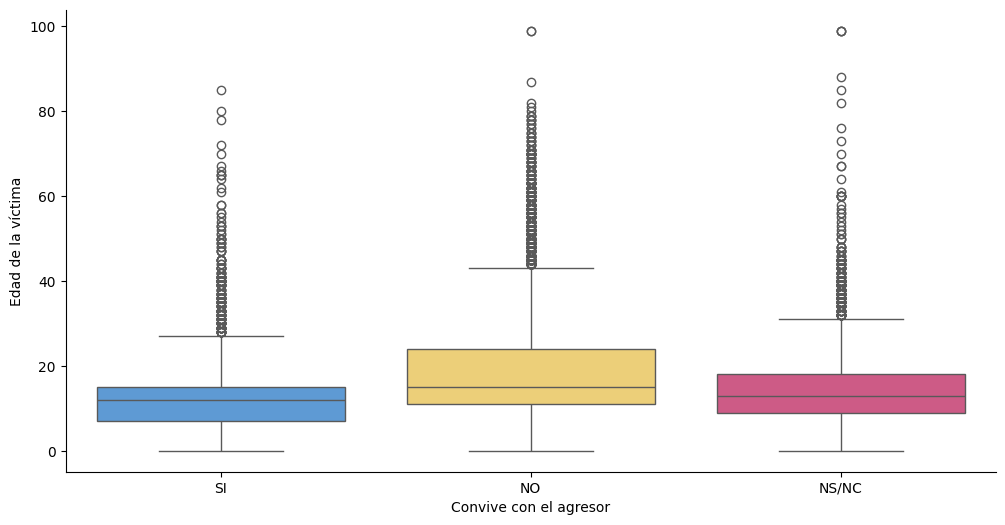
\includegraphics[scale=.4]{images/latex_boxplot_convive_edad.png}
    \caption{Distribución de la edad de la víctima según su convivencia o no con el agresor.}
    \label{boxplotsconvivenciaedad}
    \end{center}
    \end{figure}


\begin{table}[H]
    \centering
    \small
    \begin{center}
    \caption{Cuartiles de edad según categoría de \texttt{victima\_convive\_agresor}.}
    \label{cuartilesconviveedad}
    \begin{tabular}{cccc}
    \hline
    \multicolumn{1}{r}{\textbf{}} & \textbf{Convive} & \textbf{No Convive} & \textbf{ NS/NC} \\ \hline
    Q1                            & 7                    & 11                   & 9                       \\
    Media                         & 12                   & 15                   & 13                      \\
    Q3                            & 15                   & 24                   & 18                      \\
    IQR                           & 8                   & 13                   & 9                     \\ \hline
    \end{tabular}
    \end{center}
    \end{table}


Evalué también una posible relación entre la edad de la víctima, el vínculo con el agresor, y la situación de convivencia o no con este. En la figura \ref{edadconvagr} se observa la tendencia que ya se presentó en los \textit{boxplots} de \ref{boxplotsconvivenciaedad}: las medias de edades de las víctimas según sus situaciones convivenciales con el agresor son similares entre sí. Destaco, sin embargo, que para las categorías \texttt{Pareja} y \texttt{Ex-pareja de la víctima} la media de edad de las víctimas es ligeramente más alta en comparación a las otras categorías de vínculos; y que específicamente la media de edad de las víctimas que sí conviven con sus agresores es más alta que la de las que no conviven o aquellas para las que no se cuenta con datos sobre la convivencia. La media de edad también se dispara para la categoría vincular \texttt{Madrastra} en los casos en que no se tienen datos sobre la situación convivencial. Por último, quiero señalar que las medias de edad más bajas ocurren con agresores \texttt{Abuelo}, \texttt{Abuela}, \texttt{Madrastra}, y \texttt{Padre}, donde ninguna media de edad supera los 10 años en las víctimas que sí conviven con sus agresores.

\begin{figure}[H]
    \begin{center}
    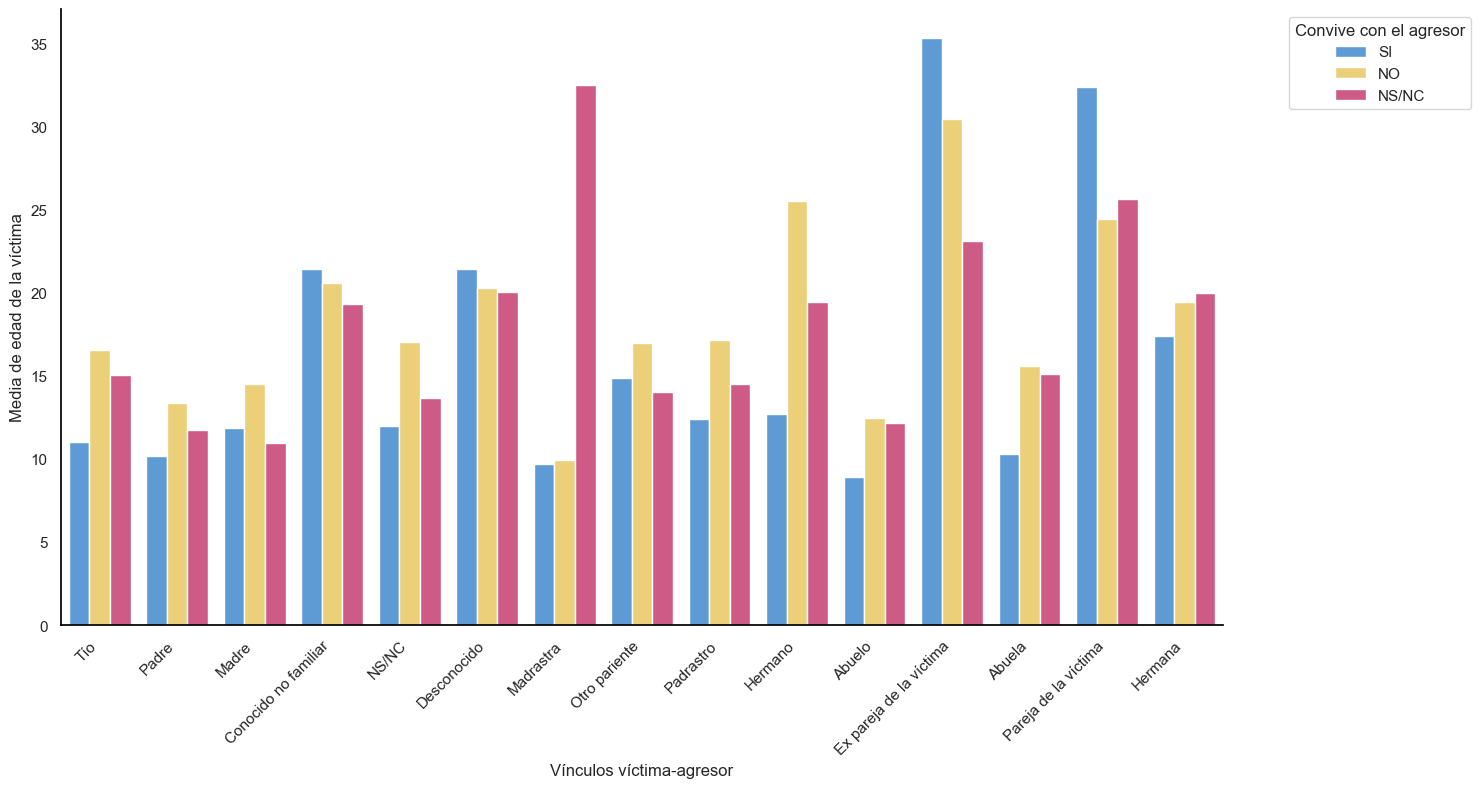
\includegraphics[scale=.4]{images/convive_edad_agresor.png}
    \caption{Edad de la víctima según su vínculo y convivencia o no con el agresor.}
    \label{edadconvagr}
    \end{center}
    \end{figure}


Por último, puse en relación \texttt{victima\_convive\_agresor} con los valores faltantes en \texttt{victima\_edad}, que representan el 9.82\%. Apliqué al conjunto de datos un filtro para incluir solamente las filas con casos vacíos de \texttt{victima\_edad}, y generé el mismo gráfico de barras de la figura \Ref{convivencia} con esos datos. El resultado, que puede verse abajo en la figura \Ref{conviveedadfaltantevic}, muestra un aumento de los casos de respuesta \texttt{NS/NC} para \texttt{victima\_convive\_agresor}. En el \textit{dataset} completo, \texttt{NS/NC} representaba el 21.19\% en \texttt{victima\_convive\_agresor}, cuando solo se observan los casos con datos faltantes de edad de la víctima, ese porcentaje sube a 57.49\%. Es decir, cuando no se tienen datos sobre la edad de la víctima, tampoco se los tiene en mayor medida sobre la situación convivencial entre la víctima y el agresor.

\begin{figure}[H]
    \begin{center}
    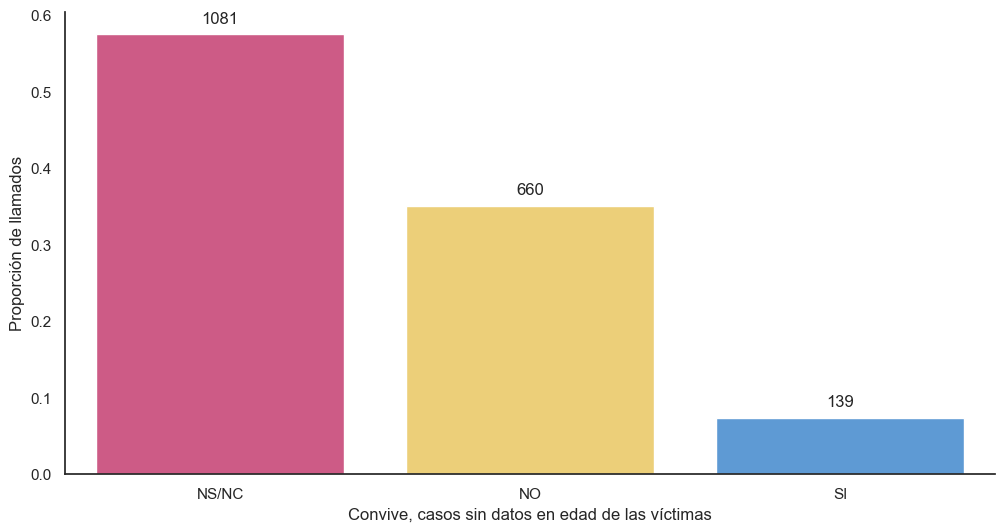
\includegraphics[scale=.4]{images/latex_convive_sd_edad_vic.png}
    \caption{Convivencia víctima-agresor en las filas de datos faltantes para \texttt{victima\_edad}.}
    \label{conviveedadfaltantevic}
    \end{center}
    \end{figure}
  


\section{Metodología}\label{met}

La alta dimensionalidad del conjunto de datos y la multiplicidad de niveles de muchas de las variables presenta desafíos para analizar relaciones multivariadas con la variable objetivo; además, puede causar problemas de procesamiento en el entrenamiento del modelo predictivo con SVM. Apliqué entonces dos métodos para reducir las dimensiones de los datos:
\begin{enumerate}
    \item \textbf{Escalamiento Multidimensional No Métrico (NMDS)}: Este método me permite generar visualizaciones en 2 dimensiones para buscar agrupamientos de las clases a predecir; y también funciona como preprocesamiento para el entrenamiento de SVM.
    \item \textbf{Reducción manual de los datos}: Eliminé, agrupé, y transformé las variables basándome en el conocimiento del dominio y el \nameref{exploración}.
\end{enumerate}

Complementé estas estrategias de reducción con dos preprocesamientos distintos para tratar los datos faltantes en las variables de edad, ya que las implementaciones que utilizo para distancia de Gower y SVM no admiten datos vacíos. Generé dos conjuntos de datos alternativos:
\begin{itemize}
    \item Conjunto A: categoricé las variables de edad\footnote{1 - 11 años = niñez; 12 - 18 años = adolescencia; 19 - 30 años = juventud; 31 - 65 años = adultez, más de 66 años = vejez.}, y clasifiqué los datos faltantes como \texttt{NS/NC}.
    \item Conjunto B: descarté la variable \texttt{llamante\_edad}, y también las filas con datos vacíos en la variable \texttt{victima\_edad}.  
\end{itemize}

La decisión sobre el conjunto B responde por un lado al supuesto de que la edad de la víctima es más relevante para la variable objetivo; y por otro lado, la edad de quien llama falta en el 44.82\%, y filtrar casos reduciría demasiado el conjunto de datos.

Finalmente evalué los efectos de estos métodos de reducción y los distintos preprocesamientos en el rendimiento del modelo SVM.

\subsection{Reordenamiento y reducción con NMDS}\label{NMDS}

NMDS, un caso particular de Escalamiento Multidimensional (MDS, por sus siglas en inglés \textit{Multidimensional Scaling}), es un método de ordenamiento que se suele utilizar para mostrar similitudes y diferencias entre los datos reorganizándolos en espacios de menor dimensión preservando el orden relativo de las distancias originales \citetext{\citealp[p. 218]{aid}}. Como su nombre lo indica, acepta matrices de distancias no métricas como entrada, y eso resulta una ventaja para el conjunto de datos multivariado con el que trabajo. 

La utilización de este método como preprocesamiento para entrenar SVM fue suscitada por los experimentos de \citeauthor{cai2019incorporating}\citeyearpar{cai2019incorporating} en el campo de la microbiología, quienes encuentran resultados con buen \textit{accuracy} aplicando esta metodología (p.69).

Implementé el método \texttt{mds} de la librería \textit{scikit-learn}\citetext{\citealp{scikit-learn}} ajustando los siguientes parámetros:

\begin{itemize}
    \item \texttt{n\_dimensions}: probé los valores entre 2 y 7.
    \item \texttt{metric}: configurado \texttt{False} para aplicar escalamiento no-métrico. 
    \item \texttt{dissimilarity}: configurado como \texttt{precomputed} para usar la matriz de distancias de Gower.
    \item \texttt{normalized\_stress}: configurado en \texttt{True} calcula el estrés para NMDS.
 \end{itemize}

Dada la naturaleza mixta de las variables del conjunto de datos, elegí la distancia de Gower para la matriz de entrada a NMDS. La similitud se calcula de a pares para variables numéricas y ordinales\footnote{Si bien \cite{podani1999extending} propone un tratamiento especial para las variables ordinales largamente utilizado hoy en día, el método que utilizo en este trabajo trata a las variables ordinales como variables numéricas como en el trabajo original de Gower. (ver \url{https://sourceforge.net/projects/gower-distance-4python/files/}).} con:

\[s_{ijk} = 1-\frac{|x_{i} - x_{j}|}{R_{k}}\]

Donde:
\begin{itemize}
    \item \(s_{ijk}\) es la similitud (o distancia) entre dos individuos o filas \(i\), \(j\) en la variable \(k\).
    \item \(R_{k}\) es el rango de \(k\).
\end{itemize}

Para variables categóricas, la similitud entre dos puntos \(i\) y \(j\) se computa de manera binaria como 0 (los valores son idénticos, mínima distancia) o 1 (no hay similitud, máxima distancia).

Luego, se calcula la matriz de similitud final con:

\[S(i,j) = \frac{\sum_{k=1}^{p}  s_{ijk}}{\sum_{k=1}^{p} \delta_{ijk}}\]

Donde \(\delta_{ijk}\) es la cantidad total de variables o la cantidad total de variables en las que puede realizarse la comparación \citetext{\citealp[p. 859-860]{gower1971general}}.

 
%\(S(i,j)\) es una matriz cuadrada con diagonal cero, que representa las distancias entre cada par de filas del conjunto de datos.

A partir de la matriz de distancias originales \textit{S}, NMDS calcula las coordenadas en un espacio reducido a n-dimensiones (en general \(n=2\) o \(n=3\) para facilitar la visualización), %obteniendo la matriz de coordenadas \(X\), %En \(X\), cada punto \(d_{ij}\) representa la distancia entre los puntos \(i\), \(j\), en el nuevo espacio reducido. Luego, se aplica a \(X\) una transformación monotónica% 
%que es 
y a su vez las transforma en una matriz con las disparidades \(\hat{d}_{ij}\). En \(\hat{d}_{ij}\) no se preservan las magnitudes de las distancias originales, pero sí se preserva el rango de ordenamiento de esas magnitudes. %\citetext{\citealp[p. 219,220]{aid}}. 
A continuación, se calcula el valor del estrés: 

\[\textit{Stress} = \sqrt{\frac{\sum_{i<j} \left( d_{ij} - \hat{d}_{ij} \right)^2}{\sum_{i<j} d_{ij}^2}}\]

El algoritmo luego itera recalculando \(d_{ij}\) y \(\hat{d}_{ij}\) para minimizar el estrés, es decir, minimizar la diferencia entre las distancias y las disparidades \citetext{\citealp[p. 117-123]{kruskal1964nonmetric}}. 

Apliqué NMDS a los conjuntos de datos A y B mencionados al comienzo de esta sección, variando los valores de \texttt{n\_components}. Generé visualizaciones con las proyecciones resultantes de \(\texttt{n\_components} = 2\) para evaluar la agrupación basada en \texttt{victima\_convive\_agresor}; y entrené modelos de SVM para cada reducción dimensional.

\subsection{Reducción manual de los datos}\label{reduccionmanual}

Eliminé 12 de las variables que describen la violencia sufrida por considerarlas poco informativas, ya que tenían tasas de respuesta positivas menores a 1\% (ver nuevamente la figuras \nameref{vssino} y \nameref{ofvsino} en la sección \nameref{datos}). 

Además, agrupé en tres categorías más amplias algunas variables que comparten dominio semántico y jurídico, como se puede ver en el cuadro \Ref{tablaagrup}:


\begin{table}[H]
    \centering
    \small
    \caption{Agrupación de variables de violencia por dominio.}
    \label{tablaagrup}
    \begin{tabular}{|c|l|}
    \hline
    \multicolumn{1}{|l|}{\textbf{Nueva variable agrupadora}} & \multicolumn{1}{c|}{\textbf{Variables agrupadas}} \\ \hline
    \multirow{4}{*}{\texttt{vs\_explotación\_sexual}}                 & \texttt{vs\_explotación\_sexual}                           \\ \cline{2-2} 
    & \texttt{vs\_explotación\_sexual\_comercial}                \\ \cline{2-2} 
    & \texttt{vs\_explotación\_sexual\_viajes\_turismo}          \\ \cline{2-2} 
    & \texttt{vs\_sospecha\_trata\_personas\_fines\_sexuales}    \\ \hline
\multirow{3}{*}{\texttt{vs\_violacion}}                          & \texttt{vs\_violacion\_via\_vaginal}                      \\ \cline{2-2} 
    & \texttt{vs\_violacion\_via\_anal}                         \\ \cline{2-2} 
    & \texttt{vs\_violacion\_via\_oral}                         \\ \hline
\multirow{2}{*}{\texttt{vs\_tentativa\_violacion}}                & \texttt{vs\_tentativa\_violacion}                     \\ \cline{2-2} 
    & \texttt{vs\_intento\_violacion\_tercera\_persona}           \\ \hline

    \end{tabular}
    \end{table}

A la hora de elegir un método de encodeo para transformar los datos para SVM, basé mi elección de \textit{one-hot enconder} en los hallazgos de \citet{udilua2023encoding} en \textit{Encoding methods for categorical data}. Comparando la performance de un modelo de SVM entrenado con distintos métodos de encodeo, el autor encuentra que \textit{one-hot encoding} resulta en modelos con mejor \textit{accuracy} de manera consistente (p.7). 

En el mismo artículo, sin embargo, el autor advierte sobre el procesamiento potencialmente costoso (en tiempo y capacidad) en que este método incurre con variables de alta cardinalidad puede resultar demasiado alto (p.7). Por lo tanto, reduje la cardinalidad de las variables con más de 5 niveles de la siguiente manera:

\begin{itemize}
    \item \texttt{llamado\_provincia} de 25 niveles a 6: \texttt{Buenos Aires}, \texttt{C.A.B.A.}, \texttt{Región Norte}, \texttt{Región Central}, \texttt{Región Patagónica}, y \texttt{NS/NC}. 
    \item \texttt{victima\_nacionalidad} de 9 niveles a 3: \texttt{Argentina}, \texttt{NS/NC}, y \texttt{Otra}. %(donde entran todas las demás nacionalidaes ya que ninguna superaba individualmente el 1\% de los llamados).
    \item \texttt{hecho\_lugar} de 17 niveles a 6: \texttt{NS/NC}, \texttt{Vivienda de la víctima}, \texttt{Vivienda del agresor}, \texttt{Redes sociales}, \texttt{Espacio/transporte público}, %(subterráneo, tren, colectivo, plaza, descampado, y calle), 
    y \texttt{Otro}. %(categoría original más residencia turística, obra en construcción, taxi, albergue transitorio, automóvil, comercio,ámbito educativo, y vivienda de un familiar).  
    \item \texttt{llamante\_vinculo} de 16 niveles a 5: \texttt{Institución}, %(hospital, comisaría, escuela, defensoría, y otras instituciones), 
\texttt{Conocido de la víctima}, %(madre, padre, abuela/o, hermana/o, otro familiar, y otro conocido), 
\texttt{Víctima}, \texttt{Agresor}, y \texttt{NS/NC}.
\item \texttt{agresor\_vinculo} de 16 niveles a 4 tomando la agrupación mostrada en la figura 7, \nameref{conocidodesconocido}: \texttt{Conocido familiar}, \texttt{Conocido no familiar}, \texttt{NS/NC}, y \texttt{Desconocido}.
\end{itemize}


El conjunto de datos resultante de la reducción manual tiene 36 variables, (el original tenía 54). En el cuadro \Ref{tab:transformaciones} del \nameref{anex} se puede ver un resumen de las variables eliminadas, agrupadas, y transformadas.

También dividí este conjunto en los tipos A y B, siguiendo el enfoque de la sección anterior, \nameref{NMDS}. 

\subsection{Modelos SVM}\label{svm}

Las máquinas de soporte vectorial son modelos de aprendizaje supervisado ampliamente utilizados para tareas de clasificación que buscan encontrar el hiperplano que mejor separa las clases en el espacio original si los datos son linealmente separables, o en un espacio transformado de mayores dimensiones cuando no lo son, maximizando el margen entre los puntos de datos más cercanos de cada clase.  

La capacidad de SVM para trabajar con datos que no son linealmente separables utilizando distintos \textit{kernel tricks} es el motivo por el que las elegí, dadas las relaciones complejas entre la variable objetivo y el resto de las variables \citetext{\citealp[p. 323-331]{aid}}. 

En la implementación y entrenamiento de los modelos de SVM, utilicé el método \texttt{svc} de \textit{scikit-learn}\citetext{\citealp{scikit-learn}} optimizando los hiperparámetros:

\begin{itemize}
    \item \texttt{kernel}: define el tipo de función para transformar el espacio de entrada.
    \item \texttt{C}: regulariza el equilibrio entre maximizar el margen entre las clases y minimizar errores de clasificación.
    \item \texttt{gamma}: un peso que controla la influencia de \textit{datapoints} individuales en la frontera de decisión del modelo.
\end{itemize}



El cuadro \Ref{modelosSVM} ofrece un resumen de los distintos conjuntos de datos para los experimentos de entrenamiento de SVM.


\begin{table}[H]
    \centering
    \small
    \caption{Preprocesamientos para entrenar modelos de SVM.}
    \label{modelosSVM}
    \begin{tabular}{|c|c|c|}
    \hline
    \textbf{Preprocesamiento}                                                                            & \textbf{Dataset} & \textbf{Especificaciones}                                                                                                                                                             \\ \hline
    \multirow{2}{*}{\begin{tabular}[c]{@{}c@{}}1. Reducción con \\ NMDS\end{tabular}}                  & A                & \begin{tabular}[c]{@{}c@{}}Variables de edad transformadas a categóricas. \\ Datos faltantes codificados como \texttt{NS/NC}\end{tabular}                                                       \\ \cline{2-3} 
                                                                                                    & B                & \begin{tabular}[c]{@{}c@{}}Solo datos completos de edad de la víctima (numérica). \\ Edad de quien llama eliminada.\end{tabular}                                                      \\ \hline
    \multirow{2}{*}{\begin{tabular}[c]{@{}c@{}}2. Reducción manual \\ con métodos mixtos\end{tabular}} & A                & \begin{tabular}[c]{@{}c@{}}Variables de edad transformadas a categóricas. \\ Datos faltantes codificados como \texttt{NS/NC}. \\ Aplicación de one hot encoder pot categorización.\end{tabular} \\ \cline{2-3} 
                                                                                                    & B                & \begin{tabular}[c]{@{}c@{}}Solo datos completos de edad de la víctima (numérica). \\ Edad de quien llama eliminada.\end{tabular}                                                      \\ \hline
    \end{tabular}
    \end{table}    



\subsubsection{Entrenamiento de SVM con reducción NMDS}

Preparé los datos comenzando por reemplazar los valores \texttt{NS/NC} en \texttt{victima\_convive\_agresor} por \texttt{NA}. Después, separé la variable objetivo \texttt{victima\_convive\_agresor} (\textit{y}) del resto de los datos \textit{X}; y quité a \textit{y} las filas vacías, guardando sus índices. Calculé a partir de X label matriz de distancias de Gower para utilizar en NMDS.

Generé distintas reducciones NMDS variando el parámetro \texttt{n\_components}. Para cada reducción, creé el conjunto de prueba ciega final de casos no vistos a partir de las filas ya transformadas de \textit{X} correspondientes a los casos con respuesta vacía en \texttt{victima\_convive\_agresor}. Dividí conjunto principal \textit{X} e \textit{y} de manera estratificada en entrenamiento (80\%) y testeo (\%20) de manera estratificada utilizando \texttt{StratifiedShuffleSplit} de \textit{scikit-learn}\citetext{\citealp{scikit-learn}} para mitigar el desbalance de las clases \texttt{SI} y \texttt{NO}.

Para el entrenamiento, implementé una búsqueda de hiperparámetros (\texttt{kernel}, \texttt{C}, \texttt{gamma}) mediante validación cruzada de 5 divisiones, evaluando el rendimiento con la métrica \texttt{f1\_weighted}. Elegí esta métrica tanto por el desbalance entre las clases (\textit{accuracy} o \textit{precision} pueden arrojar valores para la clase predominante), como para intentar garantizar un modelo que balanceara precisión y cobertura, ya que me interesa no solo predecir de manera correcta los verdaderos positivos, sino también, no dejar afuera potenciales casos positivos. Además, calculé el estrés asociado a cada reducción NMDS como una métrica adicional de evaluación.


Finalmente, probé el modelo entrenado con los mejores hiperparámetros en el conjunto ciego. Aunque no me es posible realizar una evaluación tradicional del conjunto final porque son realmente datos faltantes, comparé las proporciones de clases \texttt{SI} y \texttt{NO} entre el conjunto original con las predicciones para obtener una estimación de la performance del modelo. 


\subsubsection{Entrenamiento de SVM con reducción manual de los datos}

Para este experimento, comencé por codificar las variables. Para \texttt{llamado\_fecha\_hora}, \texttt{momento\_dia}, \texttt{estacion\_del\_año}, y las variables de edad (en el caso del conjunto A) utilicé un encoder ordinal (\texttt{OrdinalEncoder} de \textit{scikit-learn}\citetext{\citealp{scikit-learn}}) para preservar la naturaleza ordinal de los datos. En el caso del conjunto B, escalé la edad de la víctima.

Transformé las variables binarias (\texttt{SI}, \texttt{NO}), incluida la variable objetivo, asignando \texttt{SI} = 1 y \texttt{NO} = 0. Al igual que en el experimento anterior, los valores \texttt{NS/NC} en la variable objetivo los reemplacé por datos vacíos. Para el resto de las variables categóricas, utilicé \texttt{OneHotEncoder}.

Generé el conjunto de prueba ciega  de manera similar al enfoque NMDS, utilizando las filas correspondientes a casos con \texttt{NS/NC} en la variable objetivo. Entrené el modelo fue entrenado con la misma metodología de validación cruzada y búsqueda de hiperparámetros (\texttt{kernel}, \texttt{C}, \texttt{gamma}), optimizando \texttt{f1\_weighted}.


\section{Resultados}\label{resultados}

\subsection{Visualización del ordenamiento con NMDS}

Las figuras \Ref{nmds_a} y \Ref{nmds_b} muestran que en el reordenamiento en dos dimensines de los datos las categorías \texttt{SI}, \texttt{NO}, y \texttt{NS/NC} no presentan una separación clara. \texttt{SI} y \texttt{NO} aparecen mezcladas entre sí, y, por consiguiente, \texttt{NS/NC} no se agrupa distintivamente cerca de ninguna de las dos clases, ni de forma aislada. Además, los valores de estrés obtenidos en ambas configuraciones de NMDS son considerablemente altos: 0.3, cuando que un valor óptimo suele encontrarse alrededor de 0.05. 

\begin{figure}[H]
    \begin{center}
    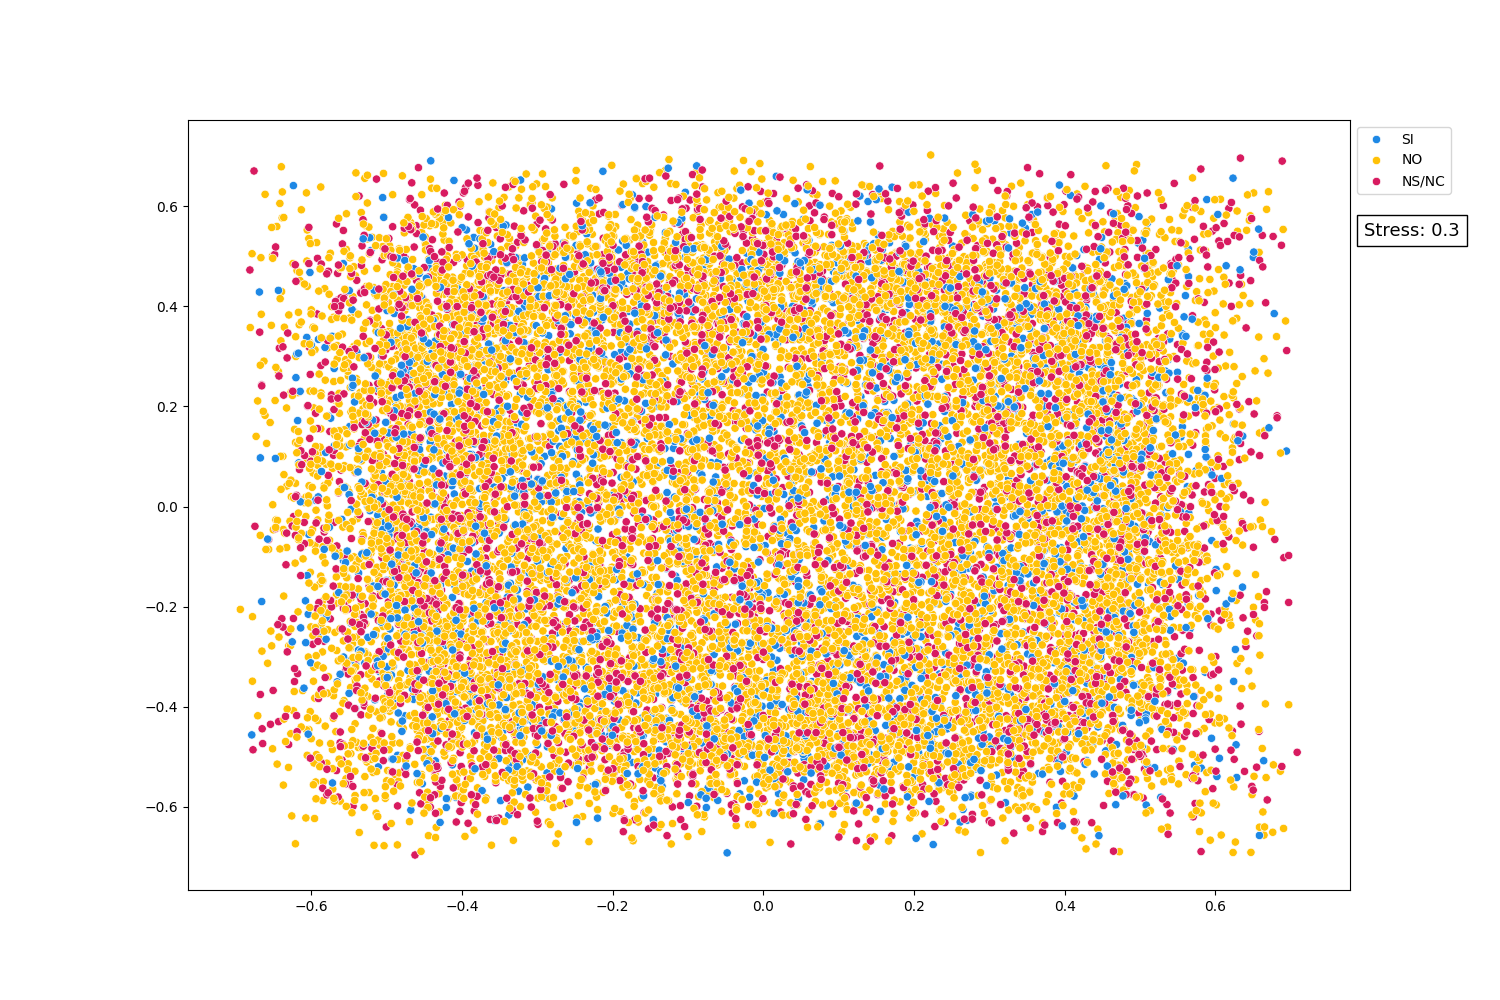
\includegraphics[scale=.4]{images/nmds_a.png}
    \caption{Visualización de los datos reducidos con NMDS - conjunto A}
    \label{nmds_a}
    \end{center}
    \end{figure}


\begin{figure}[H]
    \begin{center}
    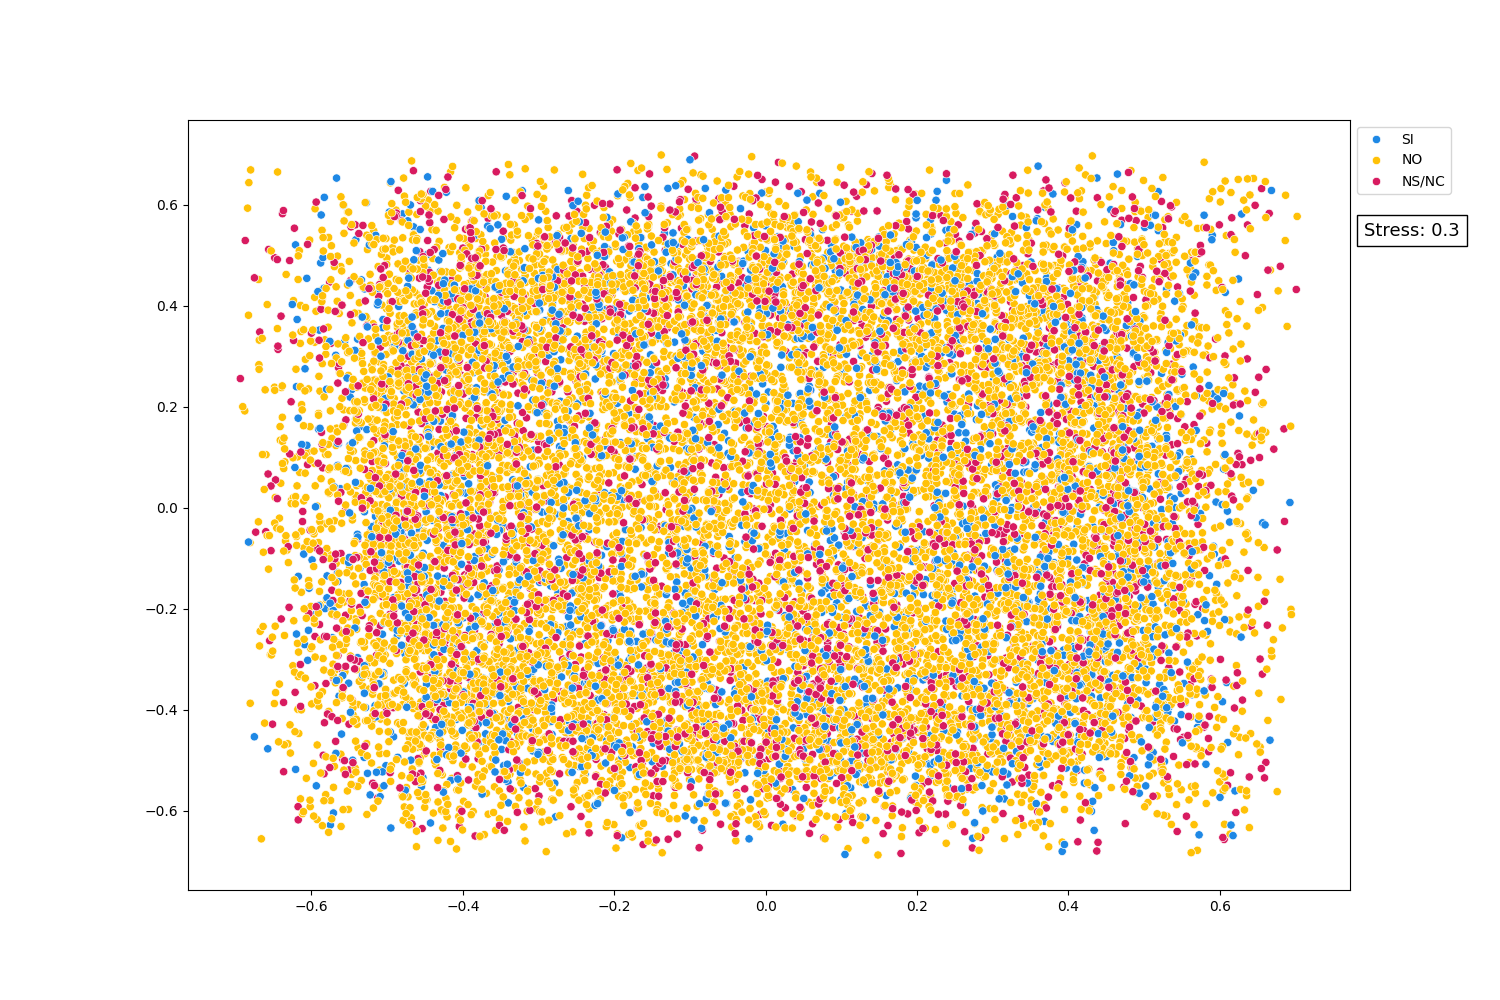
\includegraphics[scale=.4]{images/nmds_b.png}
    \caption{Visualización de los datos reducidos con NMDS - conjunto B}
    \label{nmds_b}
    \end{center}
    \end{figure}    

\subsection{Modelos predictivos de SVM}

\subsubsection{Preprocesamiento con NMDS}

Los valores de estrés para los ordenamientos aún en dimensiones \(>2\) resultaron nuevamente altos, siendo el más bajo 0.16 para 7 dimensiones.

Para los conjuntos de datos A y B, y para todas las variaciones de \texttt{n\_components}, la optimización de hiperparámetros encontró siempre los mejores resultados con:

\begin{itemize}
    \item \texttt{kernel: polynomial}
    \item \texttt{C: 0.1}
    \item \texttt{gamma: auto}
\end{itemize}

La selección del \texttt{kernel} polinomial da cuenta de la no linealidad de los datos en el espacio de entrada. El valor bajo de la penalización \texttt{C} indica una preferencia por generalizar antes que por minimizar los errores de entrenamiento. La configuración de \texttt{gamma} en \textit{auto} hace que el valor resultante para este parámetro resulte de \(\frac{1}{\texttt{n\_components}}\): \(0.5 \leq \gamma \leq \pi\), ya que \(2 \leq \texttt{n\_components} \leq 7\). 

La performance de los modelos también se igualó en ambos conjuntos de datos y para todos los \texttt{n\_components}, puede verse resumida en el cuadro \Ref{svmperfonmds} a continuación. Los modelos resultan sumamente afectados por el desbalance de clases y no generalizan bien para la clase minoritaria. Las métricas F1, cobertura, y precisión son buenas para la clase mayoritaria \texttt{NO} (0.90, 1.00, y 0.82 respectivamente), indicando que son modelos capaces de identificar correctamente la mayoría de los puntos de esta clase. Para la clase minoritaria \texttt{SI}, si bien los modelos no incurren en falsos positivos en la clasficación (de ahí la precisión de 1.0), tampoco pueden identificar correctamente nigún caso perteneciente a la clase, haciendo que la cobertura, y por lo tanto F1, sean 0.

Las métricas F1 macro (0.45) y cobertura macro (0.50), que promedian el rendimiento en ambas clases, dan cuenta del problema del desbalance de los datos. La métrica general de \textit{accuracy} por el contrario resulta engañosa por sí sola, pero su valor alto (0.82) responde al sobreajuste del modelo para la clase mayoritaria. Otro tanto sucede con la macro precisión que promedia la precisión por clase, y como comenté anteriormente, la precisión para la clase minoritaria solo es alta porque el modelo no incurre en falsos positivos.

\begin{table}[H]
    \centering
    \small
    \caption{Performance de modelos SVM utilizando NMDS como preprocesamiento.}
    \label{svmperfonmds}
    \begin{tabular}{cccccccc}
    \hline
    \multicolumn{1}{l}{\textbf{Clase}} & \multicolumn{1}{l}{\textbf{F1}} & \multicolumn{1}{l}{\textbf{Cobertura}} & \multicolumn{1}{l}{\textbf{Precisión}} & \multicolumn{1}{l}{\textbf{Macro F1}} & \multicolumn{1}{l}{\textbf{Macro Cobertura}} & \multicolumn{1}{l}{\textbf{Macro Precisión}} & \multicolumn{1}{l}{\textbf{Accuracy}} \\ \hline
    0 (NO) & 0.90 & 1.00 & 0.82 & \multirow{2}{*}{0.45} & \multirow{2}{*}{0.50} & \multirow{2}{*}{0.91} & \multirow{2}{*}{0.82} \\
    1 (SI) & 0.00 & 0.00 & 1.00 &  &  &  &  \\ \hline
    \end{tabular}
    \end{table}


Al aplicar los mejores modelos a los sets de testeo final ciegos para A y B, encontré que identificaban todos los casos como pertenecientes a la clase mayoritaria \texttt{NO}.  


\subsubsection{Preprocesamiento con reducción manual}


La optimización de hiperparámetros encontró los mejores resultados con:


\begin{multicols}{2}
\textbf{Conjunto A}
    \begin{itemize}
        \item \texttt{kernel: polynomial}
        \item \texttt{C: 1}
        \item \texttt{gamma: scale}
    \end{itemize}    
    \columnbreak
    \textbf{Conjunto B}
    \begin{itemize}
        \item \texttt{kernel: rbf}
        \item \texttt{C: 100}
        \item \texttt{gamma: auto}
    \end{itemize}
\end{multicols}    


Ambos \textit{kernels} apropiados para datos no lineales. El mejor valor del parámetro de regularización \texttt{C} es significativamente más alto que para el experimento anterior, sobre todo en el caso del conjunto B. 

Al igual que en el experimento anterior, las métricas de performance se igualaron para los modelos entrenados con cada conjunto A y B. Los resultados pueden verse en el cuadro \Ref{svmperfomanual}. En este segundo experimento el modelo resulta mejor clasificador de la clase minoritaria que en el experimento anterior mirando F1, cobertura, y precisión para \texttt{NO} (0.62, 0.54, y 0.72 respectivamente), y mantiene la buena performance para la clase mayoritaria (0.93, 0.95, y 0.90 respectivamente). Si bien la mejora es notable, las cifras alcanzadas no hablan de un modelo confiable para clasificar casos de \texttt{SI}, de hecho la cobertura parece estar cerca de una clasificación por azar. La precisión de 0.72 en \texttt{SI} es la más alta de las tres métricas para esta clase porque responde al mismo fenómeno que en el experimento anterior.


Las métricas F1 macro (0.77), cobertura macro (0.75) también mejoraron con respecto al experimento anterior. La precisión macro (0.81) y la \textit{accuracy} (0.88) responden a los mismos fenómenos que en el experimento anterior aunque esta vez la diferencia de performance por clase no es tan extrema.

\begin{table}[H]
    \centering
    \small
    \caption{Performance de modelos SVM reducción manual como preprocesamiento.}
    \label{svmperfomanual}
    \begin{tabular}{cccccccc}
    \hline
    \multicolumn{1}{l}{\textbf{Clase}} & \multicolumn{1}{l}{\textbf{F1}} & \multicolumn{1}{l}{\textbf{Cobertura}} & \multicolumn{1}{l}{\textbf{Precisión}} & \multicolumn{1}{l}{\textbf{Macro F1}} & \multicolumn{1}{l}{\textbf{Macro Cobertura}} & \multicolumn{1}{l}{\textbf{Macro Precisión}} & \multicolumn{1}{l}{\textbf{Accuracy}} \\ \hline
    0 (NO) & 0.93 & 0.95 & 0.90 & \multirow{2}{*}{0.77} & \multirow{2}{*}{0.75} & \multirow{2}{*}{0.81} & \multirow{2}{*}{0.88} \\
    1 (SI) & 0.62 & 0.54 & 0.72 &  &  &  &  \\ \hline
    \end{tabular}
    \end{table}


Al comparar las proporciones de \texttt{SI} y \texttt{NO} predichas por los mejores modelos en los sets de testeo ciegos con la proporción existente en el conjunto de datos original\footnote{Tomo los datos post procesamiento manual, sin las filas \texttt{NS/NC} en cada caso A y B.}, encontré los resultados resumidos en el cuadro a continuación:

\begin{table}[H]
    \centering
    \caption{Proporciones predichas vs. originales para cada clase.}
    \label{predichovsoriginal}
    \begin{tabular}{lcccc}
    \hline
    \multicolumn{1}{c}{\textbf{\begin{tabular}[c]{@{}c@{}}Conjunto\end{tabular}}} & \multicolumn{1}{l}{\textbf{\texttt{SI} original}} & \multicolumn{1}{l}{\textbf{\texttt{SI} predicho}} & \multicolumn{1}{l}{\textbf{\texttt{NO} original}} & \multicolumn{1}{l}{\textbf{\texttt{NO} predicho}} \\ \hline
    \textbf{A} & 0.18 & 0.09 & 0.82 & 0.91 \\
    \textbf{B} & 0.18 & 0.10 & 0.82 & 0.90 \\ \hline
    \end{tabular}
    \end{table}



\section{Conclusiones}\label{conc}

Dadas las falencias de las representaciones con NMDS (las visualizaciones que no aportaron información útil, la apariencia aleatoria de la distribución de los datos, y los valores de estrés deficientes), en el futuro podría explorar otras metodologías de reducción y visualización, como por ejemplo PCA, mediando siempre una transformación adecuada de los datos. Es posible también que en este conjunto de datos los patrones relacionados con la varaible objetivo sean demasiado complejos para ser representados en dos o tres dimensiones.

Aunque el preprocesamiento manual del dataset produjo resultados notablemente superiores en el entrenamiento de los clasificadores/imputadores de datos faltantes, ambos experimentos sufrieron el desbalance de clases y no podría decir que ningún modelo constituye una fuente confiable para la imputación de los datos.

El preprocesamiento con NMDS fue el que produjo los peores modelos. Los distintos valores de \texttt{n\_components} y las dos estrategias para manejar valores faltantes de edad no afectaron el desempeño de los modelos. El valor bajo de la regularización \texttt{C} (0.1) podría haber contribuido al sobreajuste a la clase mayoritaria en el primer experimento con NMDS. En el segundo experimento, con valores de \texttt{C} más altos (1 para el dataset A y 100 para el dataset B), el modelo funcionó mejor. Sin embargo, esto no implica que \texttt{C} sea el único factor que explica la diferencia de rendimiento, ya que durante la optimización de hiperparámetros en el primer experimento también probó valores más altos de \texttt{C} sin obtener mejores resultados.

El parámetro \texttt{gamma}, configurado como \texttt{scale} en el segundo experimento y como \texttt{auto} en el primero, parece no haber tenido un impacto significativo por sí solo.

Para trabajos futuros, considero importante implementar estrategias que mitiguen el desbalance de clases, como la generación artificial de casos de la clase minoritaria, o el sobremuestreo o el submuestreo de las clases.

A modo general, me resulta interesante también la posibilidad de cruzar datos de diferentes fuentes sobre violencia de género y violencia sexual disponibles en Argentina, como los datos de la línea 144 para denunciar violencia de género, los registros de la OVD (Oficina de Violencia Doméstica), y los datos que pudiera aportar el Observatorio de Datos de Género. 

Finalmente, en lo referente al género de víctimas y victimarios, y volviendo a un comentario hecho en la introducción, es esencial que la recolección de datos se realice con conciencia y perspectiva de género. Como señala Rita Segato en La guerra contra las mujeres (\citeyear{segato2016guerra}), la violencia sexual está dirigida hacia cuerpos femeninos o \textit{feminizados}. Esto incluye cuerpos percibidos como menores, débiles, racializados o pertenecientes a disidencias sexuales, lo cual coincide con datos que indican una mayor incidencia de violencia sexual contra hombres durante la niñez y adolescencia, cuando los sujetos son más vulnerables y, por lo tanto, feminizados \citep{contreras2016violencia,ufem_relevamiento,ferris2002world}.

A partir de estas reflexiones, propongo una pregunta para futuros estudios: si las denuncias de violencia sexual contra disidencias de género son una minoría en los datos, ¿significa esto que esas personas sufren menos violencia sexual? ¿O refleja una subrepresentación general debido a su posición como minorías sociales y su limitado acceso a la justicia?


\newpage


\bibliography{bibtex_reporte.bib}

\newpage
\section{Anexo}\label{anex}

\begin{figure}[H]
\begin{center}
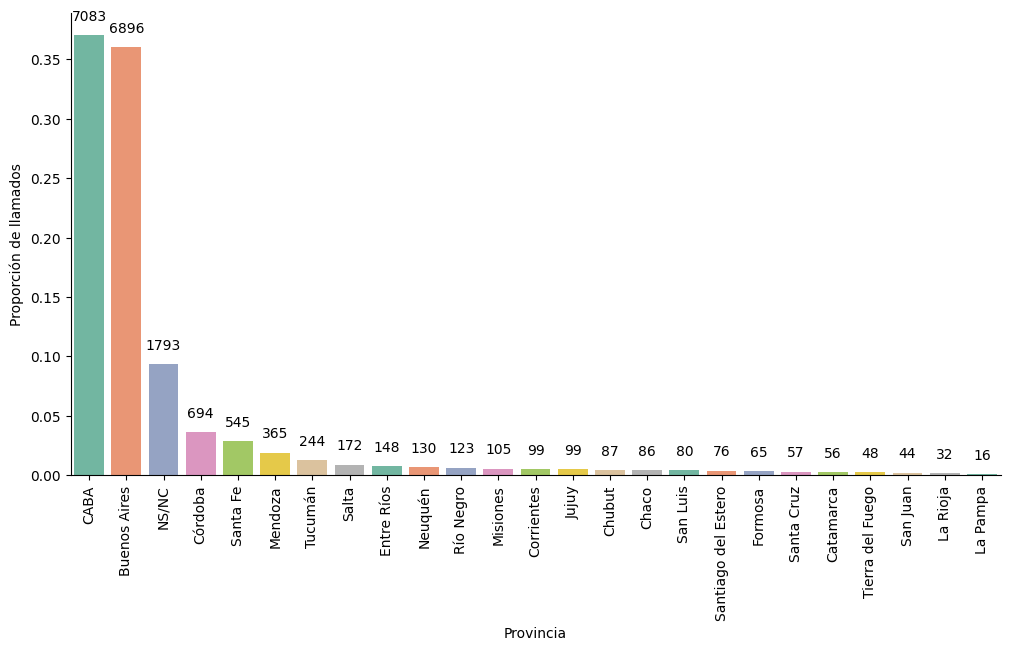
\includegraphics[scale=.4]{images/latex_llamados_por_provincia.png}
\caption{Llamados por provincia.}
\label{provincia}
\end{center}
\end{figure}

\begin{figure}[H]
\begin{center}
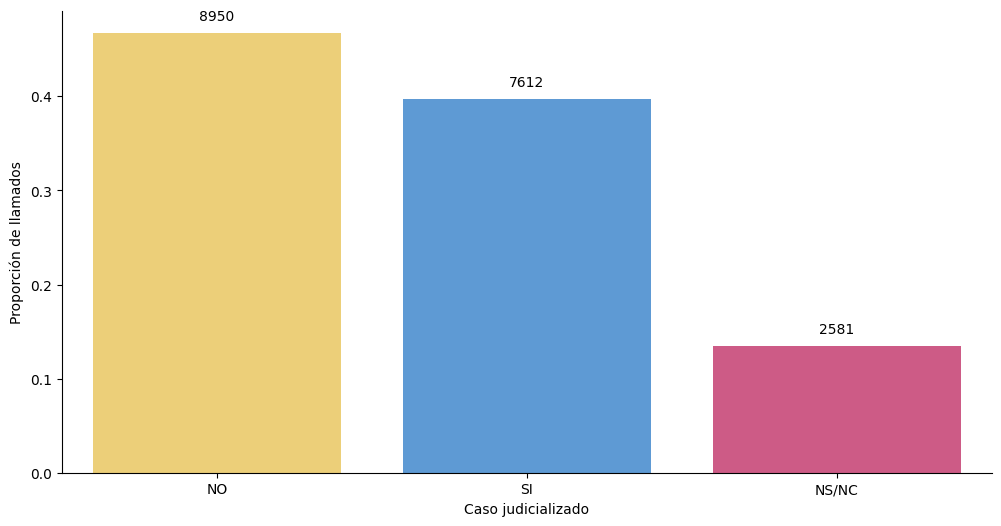
\includegraphics[scale=.4]{images/latex_caso_judicializado.png}
\caption{Caso judicializado.}
\label{casojudicializado}
\end{center}
\end{figure}


\begin{figure}[H]
\begin{center}
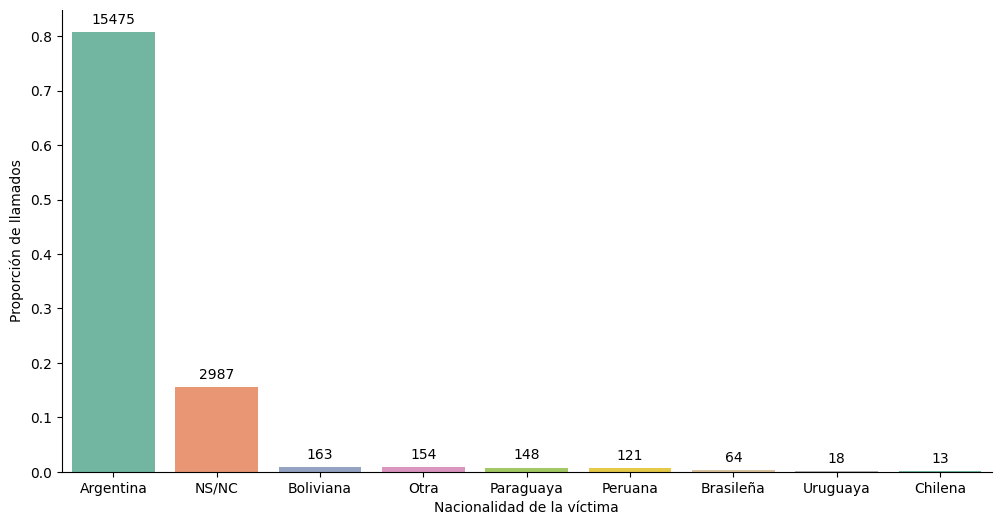
\includegraphics[scale=.4]{images/latex_nacionalidad_victima.png}
\caption{Nacionalidad de las víctimas.}
\label{nacionalidad}
\end{center}
\end{figure}



\begin{figure}[H]
\begin{center}
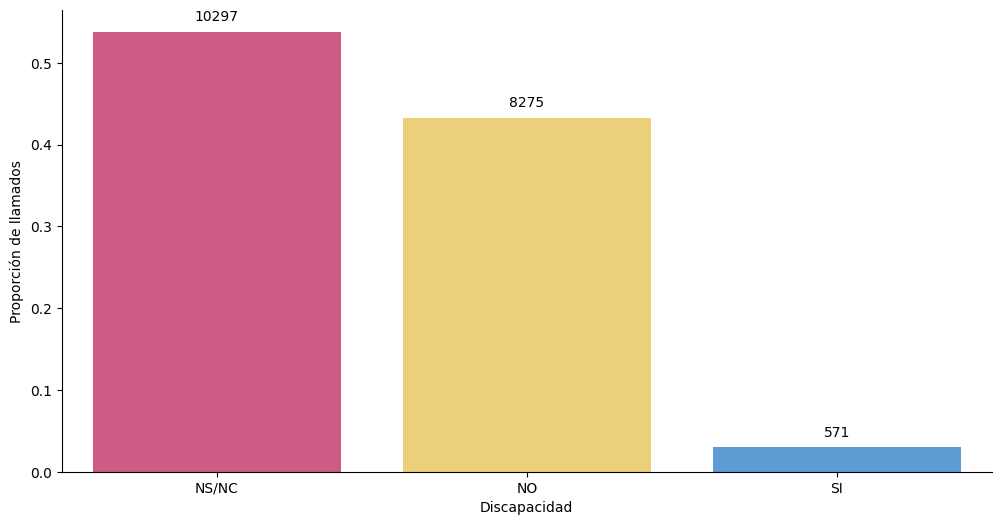
\includegraphics[scale=.4]{images/latex_victima_discapacidad.png}
\caption{Presencia de discapacidad en las víctimas.}
\label{discapacidad}
\end{center}
\end{figure}



\begin{figure}[H]
\begin{center}
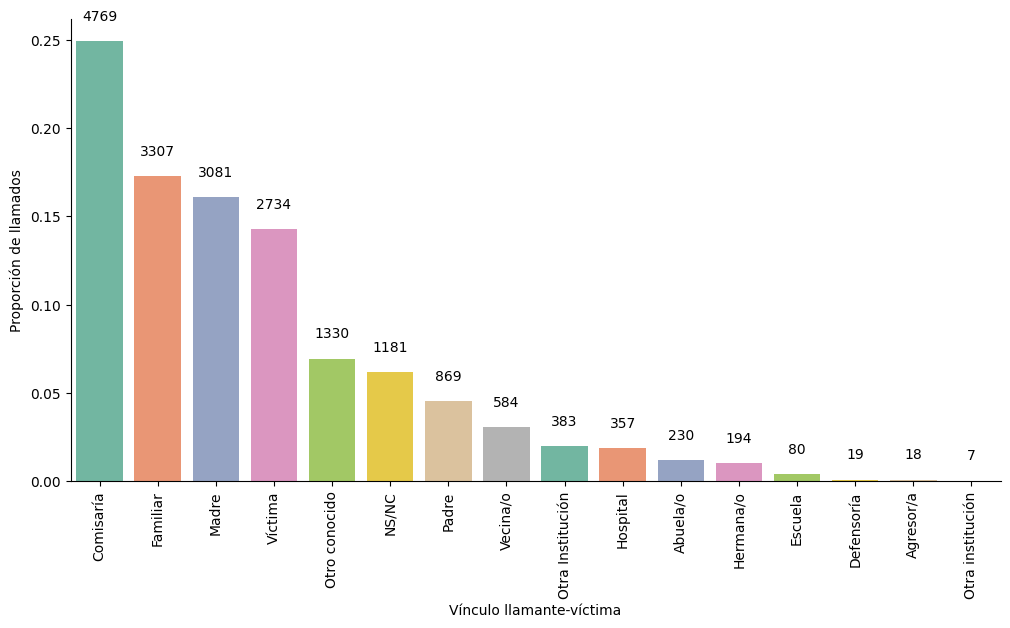
\includegraphics[scale=.4]{images/latex_vinculo_llamante.png}
\caption{Vínculos víctima-llamante.}
\label{vinculollamante}
\end{center}
\end{figure}


\begin{table}[H]
    \centering
    \small
    \caption{Resumen de transformaciones de variables.}
    \label{tab:transformaciones}
    \begin{tabular}{|l|l|l|}
    \hline
    \multicolumn{1}{|c|}{\textbf{\textit{Dataset} original}} & \multicolumn{1}{c|}{\textbf{\textit{Dataset} reducido}} & \multicolumn{1}{c|}{\textbf{Transformación}}\\ \hline
    \begin{tabular}[c]{@{}l@{}}\texttt{vs\_amenazas\_verbales\_contenido\_sexual}, \\ \texttt{vs\_existencia\_facilitador\_corrupcion\_nnya}, \\ \texttt{vs\_eyaculacion\_partes\_cuerpo}, \\ \texttt{ofv\_intento\_ahorcar}, \texttt{ofv\_intento\_quemar}, \\ \texttt{ofv\_intento\_ahogar}, \texttt{ofv\_amenaza\_muerte}, \\ \texttt{ofv\_uso\_sustancias\_psicoactivas}, \\ \texttt{ofv\_intento\_privacion\_libertad}, \\ \texttt{ofv\_privacion\_libertad}, \\ \texttt{ofv\_uso\_animal\_victimizar}, \texttt{ofv\_intento\_matar} \\ \end{tabular} & \texttt{Eliminadas} & No informativas (\textless 1\%) \\ \hline 
    \begin{tabular}[c]{@{}l@{}}\texttt{vs\_explotación\_sexual}, \\ \texttt{vs\_explotación\_sexual\_comercial}, \\ \texttt{vs\_explotación\_sexual\_viajes\_turismo}, \\ \texttt{vs\_sospecha\_trata\_personas\_fines\_sexuales}\end{tabular} & \texttt{vs\_explotación\_sexual} & Agrupadas por dominio \\ \hline
    \begin{tabular}[c]{@{}l@{}}\texttt{vs\_violacion\_via\_vaginal}, \\ \texttt{vs\_violacion\_via\_anal}, \\ \texttt{vs\_violacion\_via\_oral}\end{tabular} & \texttt{vs\_violacion} & Agrupadas por dominio \\ \hline
    \begin{tabular}[c]{@{}l@{}}\texttt{vs\_tentativa\_violacion}, \\ \texttt{vs\_intento\_violacion\_tercera\_persona}\end{tabular} & \texttt{vs\_tentativa\_violacion} & Agrupadas por dominio \\ \hline
    \texttt{llamado\_provincia} & \begin{tabular}[c]{@{}l@{}}\texttt{Buenos Aires}, \texttt{C.A.B.A.}, \\ \texttt{Región Norte}, \texttt{Región Central}, \\ \texttt{Región Patagónica}, \texttt{NS/NC}\end{tabular} & Reducción de niveles \\ \hline
    \texttt{victima\_nacionalidad} & \begin{tabular}[c]{@{}l@{}}\texttt{Argentina}, \texttt{Otra}, \\ \texttt{NS/NC}\end{tabular} & Reducción de niveles \\ \hline
    \texttt{hecho\_lugar} & \begin{tabular}[c]{@{}l@{}}\texttt{NS/NC}, \texttt{Vivienda víctima}, \\ \texttt{Vivienda agresor}, \texttt{Redes sociales}, \\ \texttt{Espacio/transporte público}, \texttt{Otro}\end{tabular} & Reducción de niveles \\ \hline
    \texttt{llamante\_vinculo} & \begin{tabular}[c]{@{}l@{}}\texttt{Institución}, \texttt{Conocido víctima}, \\ \texttt{Víctima}, \texttt{Agresor}, \texttt{NS/NC}\end{tabular} & Reducción de niveles \\ \hline
    \texttt{agresor\_vinculo} & \begin{tabular}[c]{@{}l@{}}\texttt{Conocido familiar}, \\ \texttt{Conocido no familiar}, \\ \texttt{Desconocido}, \texttt{NS/NC}\end{tabular} & Reducción de niveles \\ \hline
    \end{tabular}
\end{table}



\end{document}